\documentclass[11pt,a4paper]{article}
\usepackage{fontspec}
\setmainfont{TeX Gyre Pagella}
\newfontfamily\headfont{Inter}[UprightFont=*-ExtraBold,BoldFont=*-ExtraBold,Extension=.otf,Path=/usr/share/fonts/opentype/inter/]
\usepackage[a4paper,margin=2.3cm]{geometry}
\usepackage{graphicx,booktabs,float,caption,array,xcolor,longtable}
\usepackage{xurl}
\usepackage[hidelinks]{hyperref}
\usepackage{titlesec}
\usepackage[round]{natbib}
\usepackage{setspace}
\setstretch{1.05}
\renewcommand{\topfraction}{0.9}
\renewcommand{\bottomfraction}{0.8}
\renewcommand{\textfraction}{0.1}
\renewcommand{\floatpagefraction}{0.75}
\setlength{\parindent}{0pt}
\setlength{\parskip}{0.55em}
\titleformat{\section}{\headfont\Large}{\thesection}{0.8em}{}
\titleformat{\subsection}{\headfont\large}{\thesubsection}{0.8em}{}
\captionsetup{font=small,labelfont=bf}
\urlstyle{same}
\hypersetup{pdftitle={The Peutinger Table Against a Modern Map},pdfauthor={Tristan Hotham}}

\begin{document}
\begin{center}
{\Large\bfseries The Peutinger Table Against a Modern Map\par}
\vspace{0.4em}
{\large Shape, space and distance on a Roman road map:\\465 places located on the scroll and 3,523 road legs measured\par}
\vspace{1.2em}
{\large Tristan Hotham\par}
\vspace{0.3em}
{\small Independent researcher\\
ORCID: 0000-0003-4931-9349\\
DOI: https://doi.org/10.5281/zenodo.23882605\par}
\vspace{0.8em}
2026
\end{center}

\begin{quote}
\small
\begin{center}\textbf{Abstract}\end{center}
The Peutinger Table (Tabula Peutingeriana), a medieval copy of a Roman road map, compresses the world from Britain to India into a strip of parchment about 6.75 m long and 34 cm high, yet records the distance between road stations. I combine the OmnesViae dataset of the Tabula (2,762 stations and 2,971 legs on the surviving sheets, after Talbert's identifications) with 465 places located by eye on Konrad Miller's 1887 facsimile and with road distances along the Itiner-e network. The figures on the map are not labelled with a unit; measured on the ground, one unit covers a median 1.41 km in a straight line outside Gaul and 2.15 km in Aquitania, Lugdunensis, Belgica and the Germanies, a ratio of 1.52, consistent with Roman miles and Gallic leagues of one and a half miles. Converted accordingly, the written distances fall between the straight line (median 0.96 of the figure) and the mapped road (median 1.10); 53\% of 1,558 legs agree with the road to within 25\%, and long journeys from Rome agree to within a few per cent in the west and about an eighth in the east. The shape, by contrast, is compressed 10.9 times more north to south than east to west (12.6 km per cm against 137.5), with regions laid on their sides; Italy receives 2.6 times its share of land. Rome lies 35.4\% of the way along the surviving strip; it would be central only if about 3.3 sheets were lost at the western end. The surviving sheets record about 79,414 km of road, 3,530 days on foot.

\textbf{Keywords:} Tabula Peutingeriana; Roman roads; historical cartography; map distortion; itineraries; Itiner-e
\end{quote}

\section{Introduction}
The Peutinger Table is a copy, made around 1200, of a late Roman map of the road network of the Roman world and beyond \citep{talbert}. It survives in Vienna as eleven parchment sheets joined into a single strip; a first sheet, which showed most of Britain and Spain, is lost. The map is famously distorted: seas are thin ribbons, peninsulas lie along the strip, and the whole known world is pressed into a band roughly twenty times as long as it is high. At the same time it is a working itinerary, drawing roads as lines with a kink at each station and writing beside each leg the distance to the next.

This study asks how wrong the shape is and how right the numbers are. Specifically: which units the figures are in, and how well they match distances measured today; how stretched the map is east to west against north to south, overall and region by region; which regions get the most space; where Rome falls on the strip; and how much road, and how many days of travel, the surviving sheets record. The paper accompanies an interactive comparison of the scroll and a modern map (\url{https://maps.tristanhotham.com/peutinger/}).

\section{Data}
\textbf{OmnesViae.} The road data come from the JSON-LD export of OmnesViae \citep{omnesviae}, a route planner by Ren\'e Voorburg built on the Tabula and on Talbert's identifications \citep{talbert}, with coordinates linked to Pleiades \citep{pleiades}. It lists 3,322 stations (one duplicated) and 3,523 legs. Each station has its name as written on the map, often a modern and classical name, coordinates and a symbol code; each leg has its two ends, the written figure (missing for 251) and flags for reconstruction, sea, mountains and rivers. OmnesViae fills the lost western sheet with 560 stations from the Antonine Itinerary; I treat these 552 reconstructed legs separately. 2,103 surviving stations have coordinates. As a check, 94\% of the 2,004 stations whose name matches a precisely located Pleiades place lie within 10 km of it.

\textbf{The facsimile.} Konrad Miller's 1887 facsimile of the whole map \citep{miller}, 26,381 by 2,014 pixels as used, public domain. The painted strip is 25,565 pixels long; the joins between the eleven sheets are marked by rules in the margin.

\textbf{Roads, provinces and outlines.} Road distances use the Itiner-e network of Roman roads \citep{itinere} as prepared in an earlier study \citep{romanroads}: 299,171 km of road sections as a graph. Provinces of about AD 117 come from the Digital Atlas of the Roman Empire \citep{dare}; coastlines from Natural Earth \citep{naturalearth}. Travel speeds are those given by English Wikipedia \citep{wiki}.

\section{Methods}
\subsection{Locating places on the scroll}
No table of positions on the Tabula exists, so I read the facsimile at full resolution sheet by sheet and recorded the pixel position of 465 stations, at the station's picture where it has one and otherwise at the start of its label, matching each to its OmnesViae entry by its written name. 433 were read clearly and 32 with some doubt. Every sheet has at least 13. The sample favours legible and well-known places and is thinner in the far east, where the map has fewer stations.

\subsection{Units and distances}
Each leg is assigned a unit zone by the province of its first station: leagues in Aquitania, Lugdunensis, Belgica, Germania Inferior and Germania Superior, the area beyond Lyon where the map notes ``usque hic legas''; an unknown unit in Persia, Central Asia and India; Roman miles elsewhere. Figures are converted at 1.48 km per mile and 2.22 km per league. The straight-line distance is the great-circle distance between the OmnesViae coordinates. The road distance places each station on the nearest Itiner-e road section within 5 km and takes the shortest path along the network between the two points, keeping it only when it is at most twice the straight line plus 10 km. Agreement is measured by the ratio of measured to stated km.

\subsection{Shape, stretch and space}
For the whole strip, I compare the east-west and north-south spans of the located places with the length and height of the parchment. For each region (groups of provinces, plus three regions beyond the frontier) with at least 8 located places, I fit an affine map from local east and north kilometres to scroll pixels by least squares. Its singular values give the scale in the most and least stretched ground directions; their ratio is the region's stretch, independent of how the region is turned. The ground direction drawn along the scroll from left to right is also recorded. For space, each pixel of the painted strip (at a tenth of full resolution) is assigned to the region of its nearest located place; a region's share of the scroll is compared with its share of the land of the provinces. A smooth thin-plate surface through the located places is used to carry modern coastlines onto the scroll and to draw on the modern map where each sheet join falls; these are illustrations, not measurements.

\subsection{Rome, totals and journeys}
Rome's position is its distance from the left edge of the painted strip over the strip's length; lost sheets are modelled as sheets of the median surviving width added at the western end. Totals add the written figures of the surviving legs. Journeys from Rome are shortest paths over all legs weighted by the written distance; 249 legs without a figure are weighted by their road distance, their straight-line distance times 1.13 (the median ratio of road to straight line), or a typical leg of 23.7 km. The map draws no sea crossings, so neither do the routes. Days use 22.5 km a day on foot, 45 by cart and 80 by courier relay \citep{wiki}.

\section{Results}
\subsection{The two maps}
Figure~\ref{fig:maps} sets the located places on the scroll beside the same places today. West to east along the strip follows west to east on the ground closely: the rank correlation of longitude with position along the scroll is 0.98, while that of latitude with height on the scroll is only 0.74.

\begin{figure}[tbp]\centering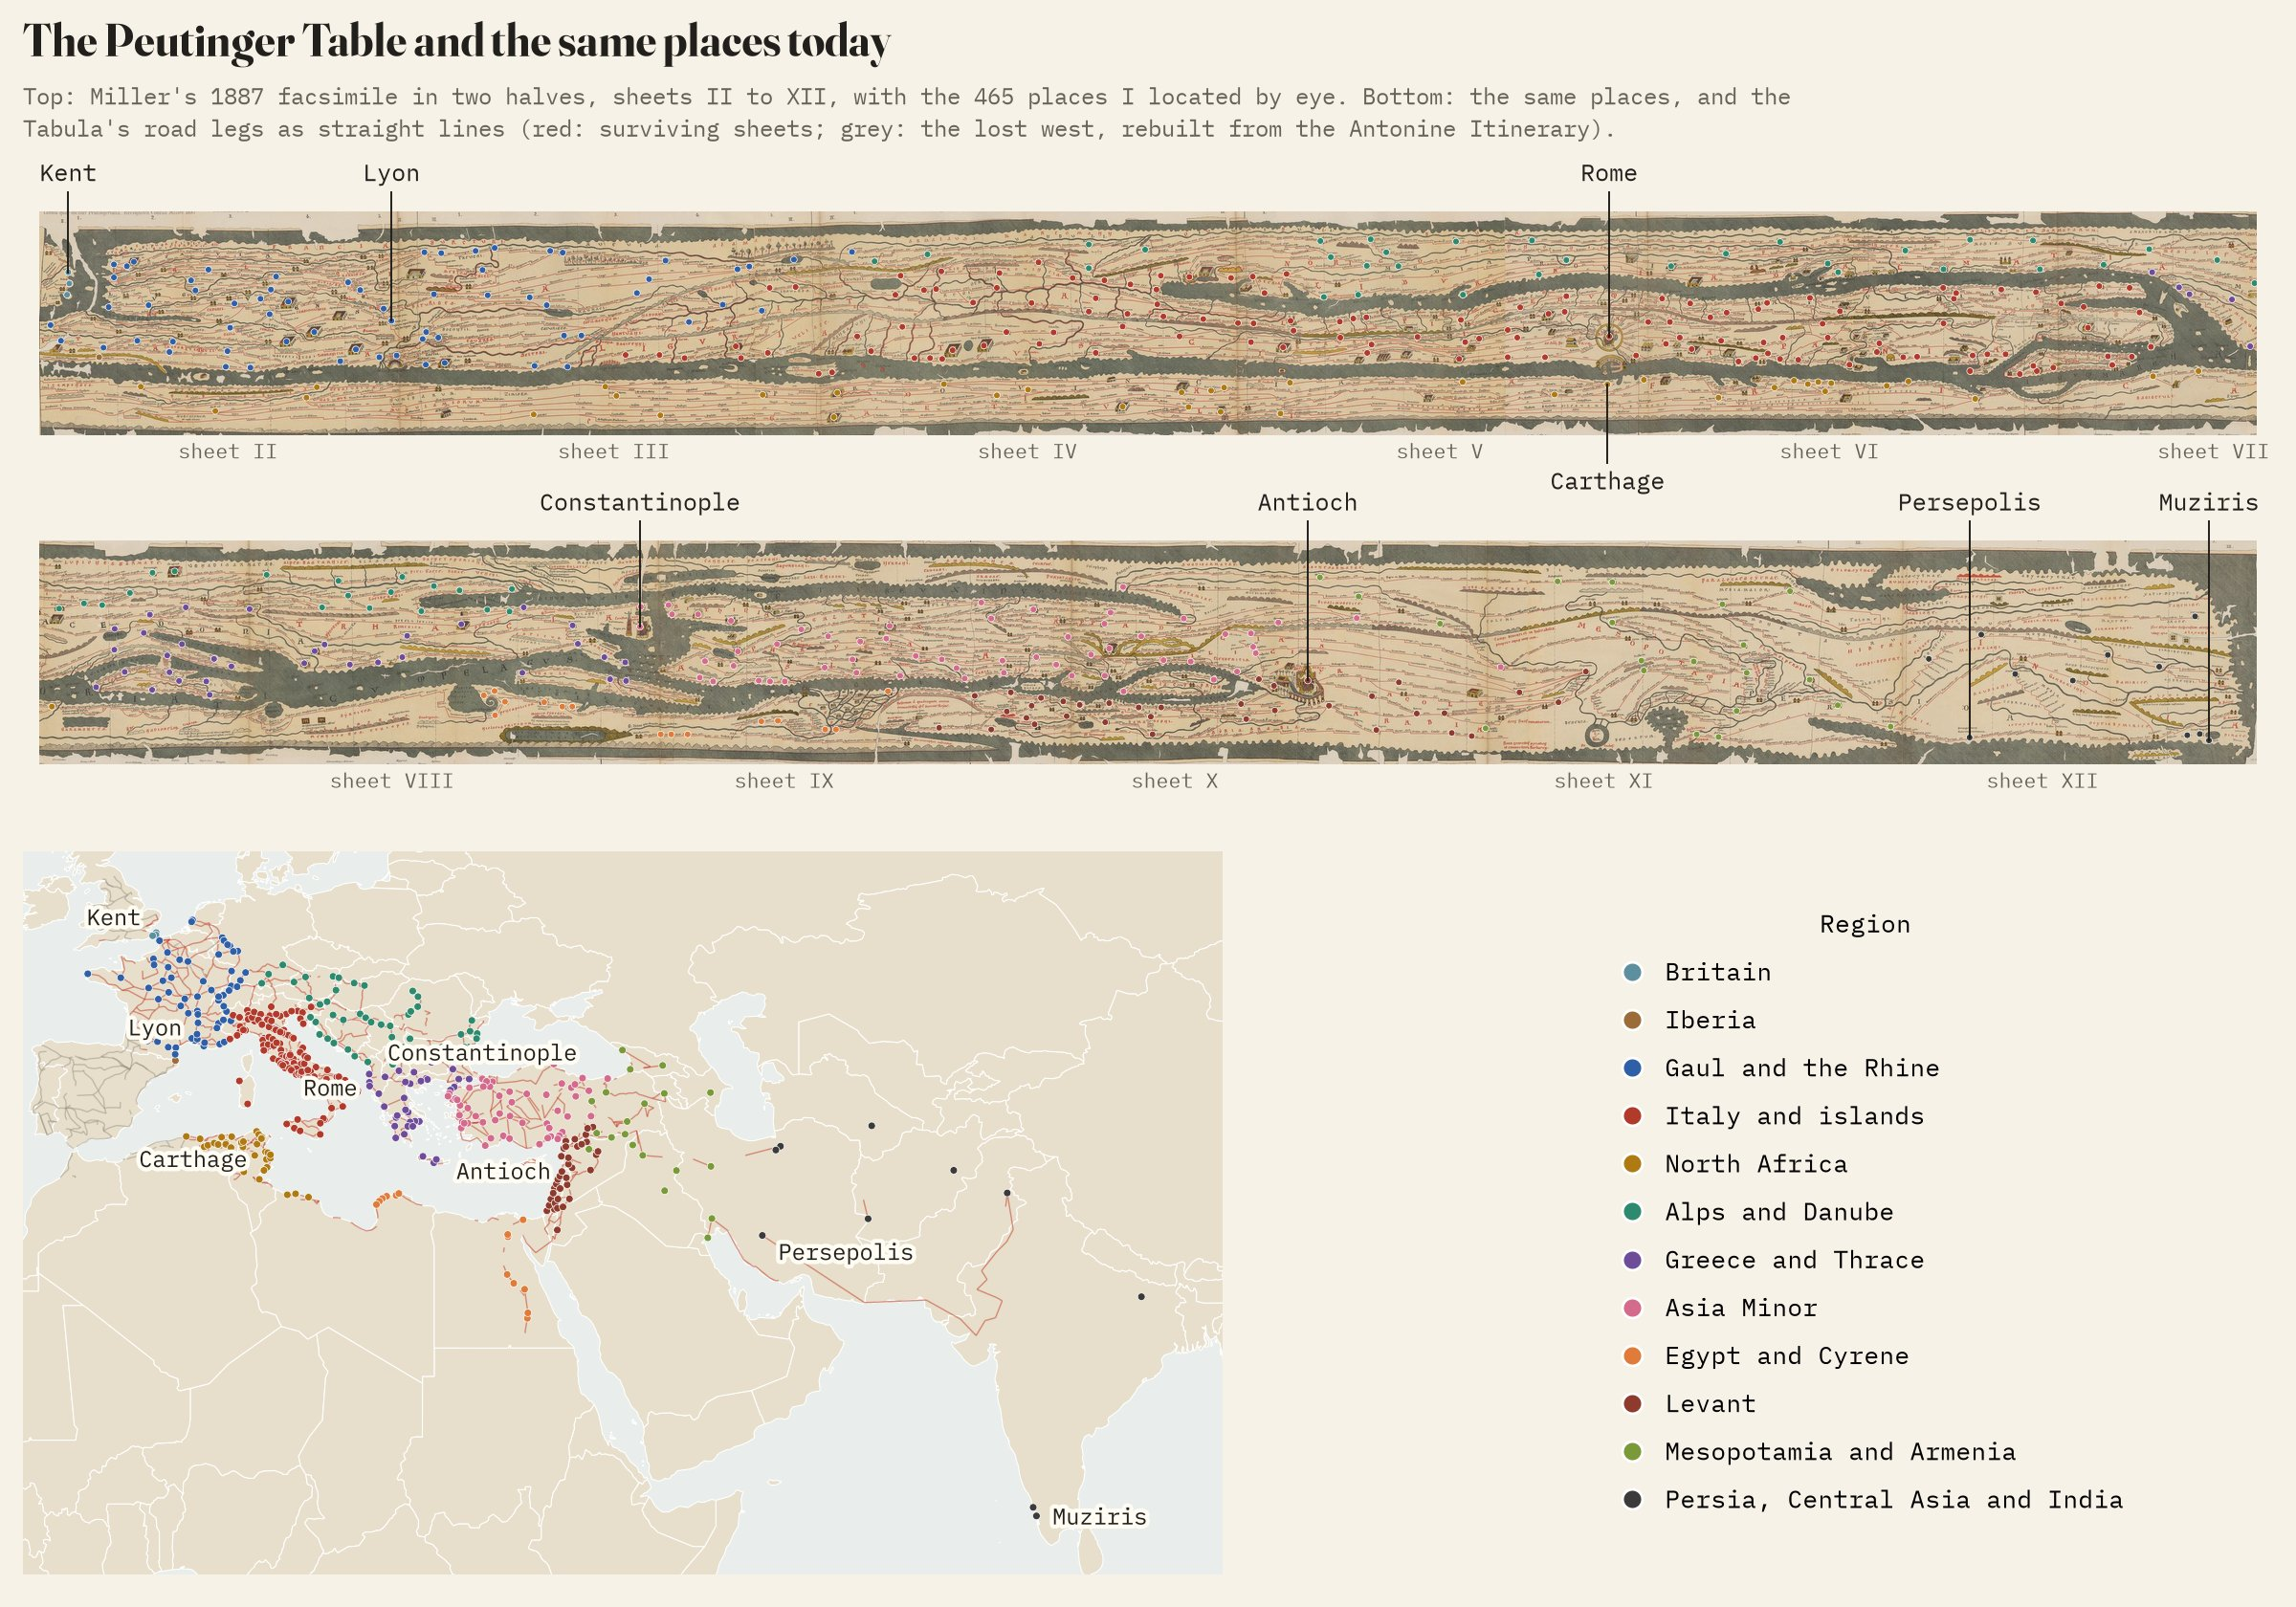
\includegraphics[width=\textwidth]{f_maps.jpg}
\caption{The located places on Miller's facsimile, in two halves (top), and on a modern map with the Tabula's legs (bottom).}\label{fig:maps}\end{figure}

\subsection{Units}
Outside the league zone, one written unit covers a median 1.41 km in a straight line and 1.64 km along the road (1,488 legs). In the league zone the figures are 2.15 and 2.34 (279 legs), 1.52 times as much in a straight line and 1.43 times along the road. Narbonensis, the Mediterranean province of Gaul, behaves like Italy (1.44). Read as miles, the league-zone legs would be 1.58 times shorter than the road; read as leagues, the ratio is 1.05 (Figure~\ref{fig:units}). In the far east only 27 legs can be measured, and one unit ranges from 0.8 to 18.7 km: 8 look like miles, 9 like parasangs of about five to seven kilometres, and the Indian legs (median 7.2 km per unit) fit no single unit.

\begin{figure}[tbp]\centering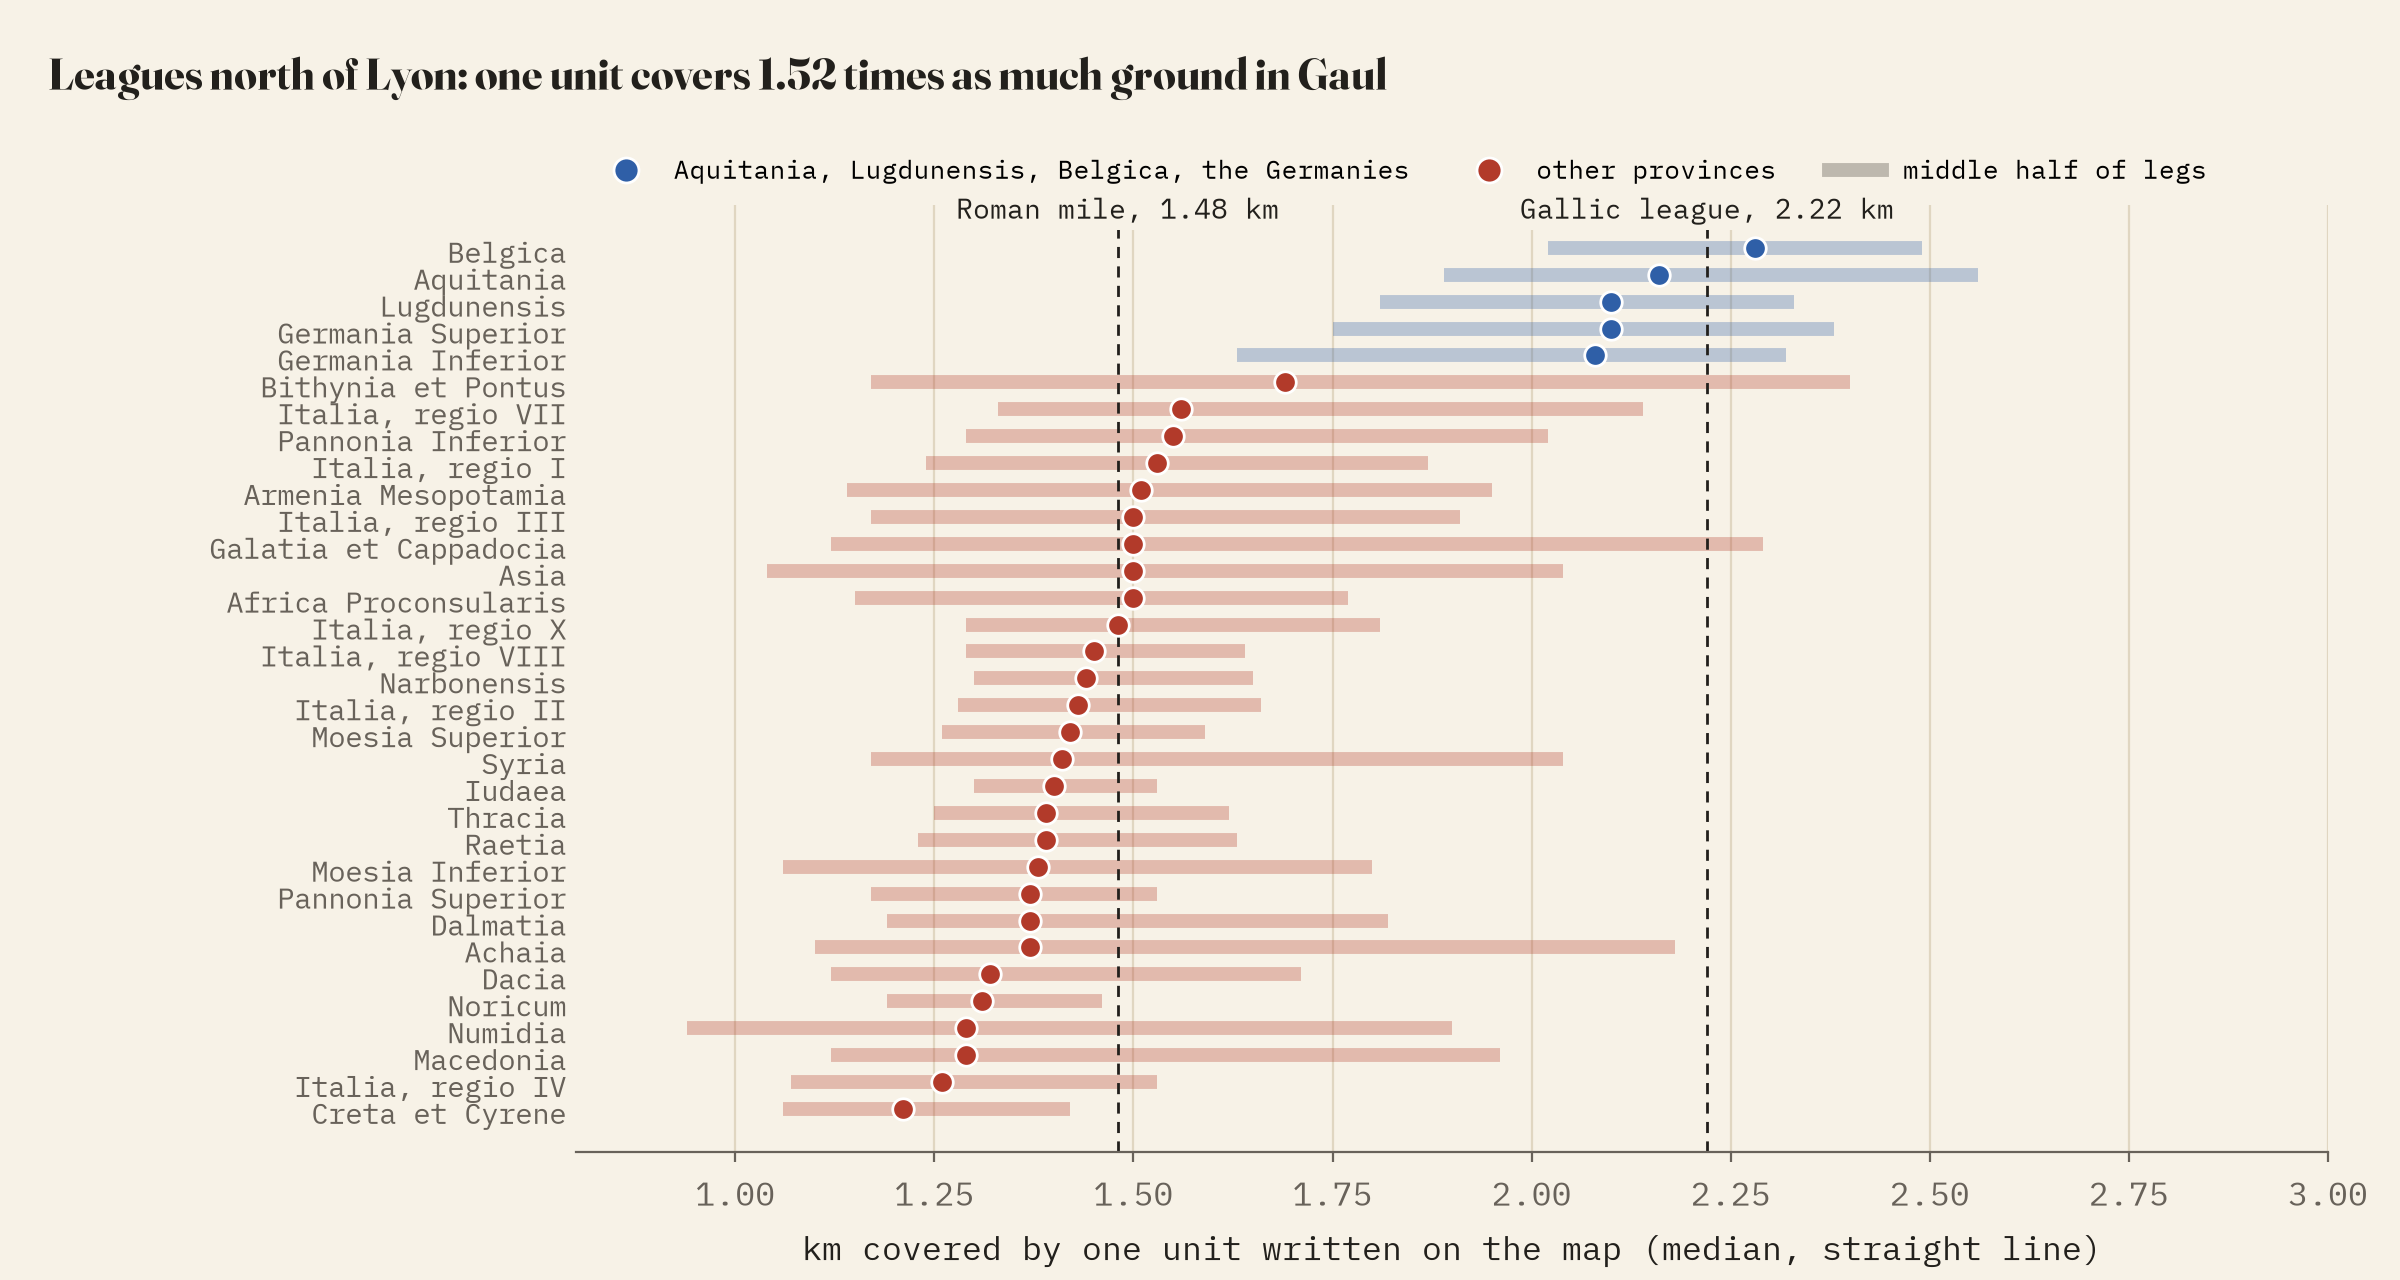
\includegraphics[width=\textwidth]{f_units.png}
\caption{Kilometres per written unit, by province (median straight-line distance per unit, with the middle half of legs).}\label{fig:units}\end{figure}

\subsection{Distances}
Converted, the written distances sit between the straight line and the road (Figure~\ref{fig:distance}). For 1,767 surviving legs in the mile and league zones the median straight line is 0.96 of the stated distance; for the 1,558 with a road distance the median road is 1.10 (middle half 0.93 to 1.41). 52.7\% of legs agree with the road to within 25\%, 70.0\% to within 50\%, and 14.3\% are off by more than a factor of two, the kind of error a dropped or doubled numeral or a misattached road would produce. The rank correlation of stated with road distance is 0.71. Over long journeys errors cancel: from Rome, the Tabula's own figures give 1,487 km to Cologne against 1,444 km along Itiner-e, 1,120 against 1,038 to Vienna and 2,081 against 2,335 to Constantinople; to Antioch and Jerusalem they run about an eighth short (2,980 against 3,411, 3,499 against 4,031).

\begin{figure}[tbp]\centering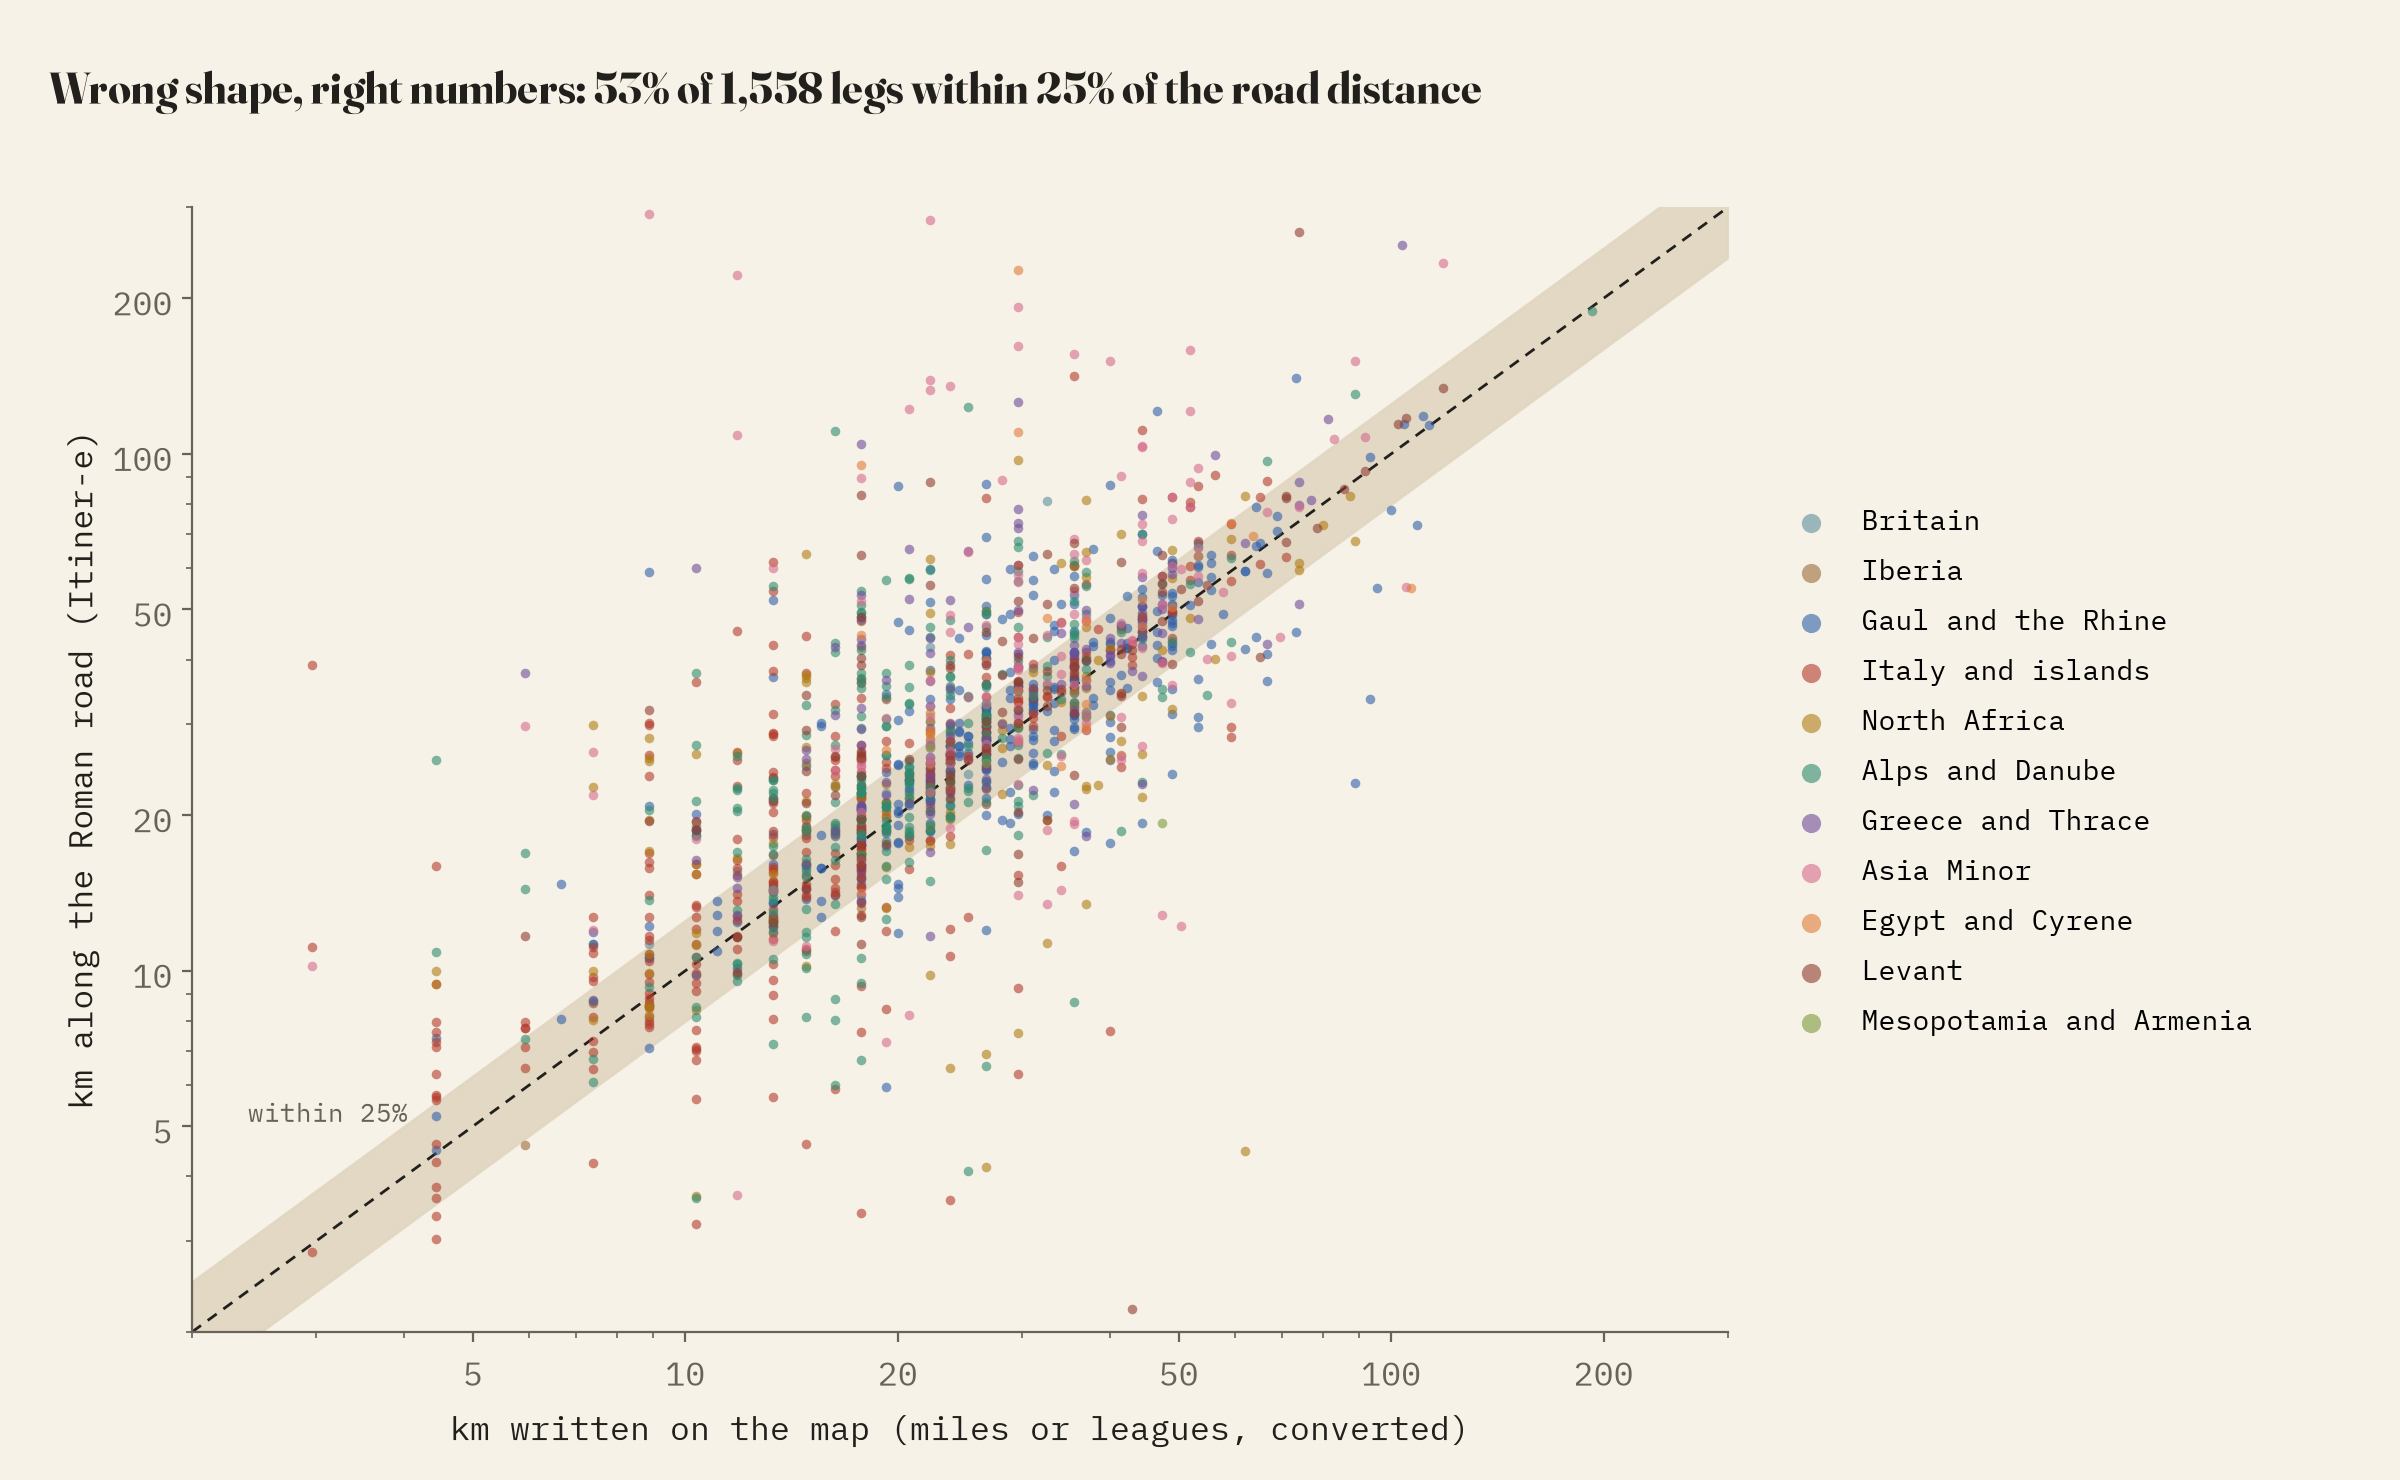
\includegraphics[width=\textwidth]{f_distance.png}
\caption{Stated against road distance for each surviving leg (log scales). The band is agreement to within 25\%.}\label{fig:distance}\end{figure}

\subsection{Shape and stretch}
The located places span about 8,526 km east to west and 4,676 km north to south, a ratio of 1.82; the painted strip is 20.9 times as long as it is high. One centimetre of parchment therefore stands for 12.6 km east to west and 137.5 km north to south, a compression of 10.9. Region by region (Table~\ref{tab:regions}, Figure~\ref{fig:stretch}), North Africa is the most stretched (55.4), then the Alps and Danube (21.3), Egypt and Cyrene (18.7), Greece and Thrace (11.1) and Italy (10.2); Mesopotamia (2.1) and Persia and India (1.7) the least, where the map places few names loosely. Italy and North Africa are both laid along the strip from north-west to south-east (ground bearings of 132 and 139 degrees). Bending Natural Earth's coastline onto the scroll through the located places (Figure~\ref{fig:warp}) puts the real Adriatic and Tyrrhenian coasts on the Tabula's seas; Figure~\ref{fig:joins} shows where the sheet joins fall on the ground.

\begin{figure}[tbp]\centering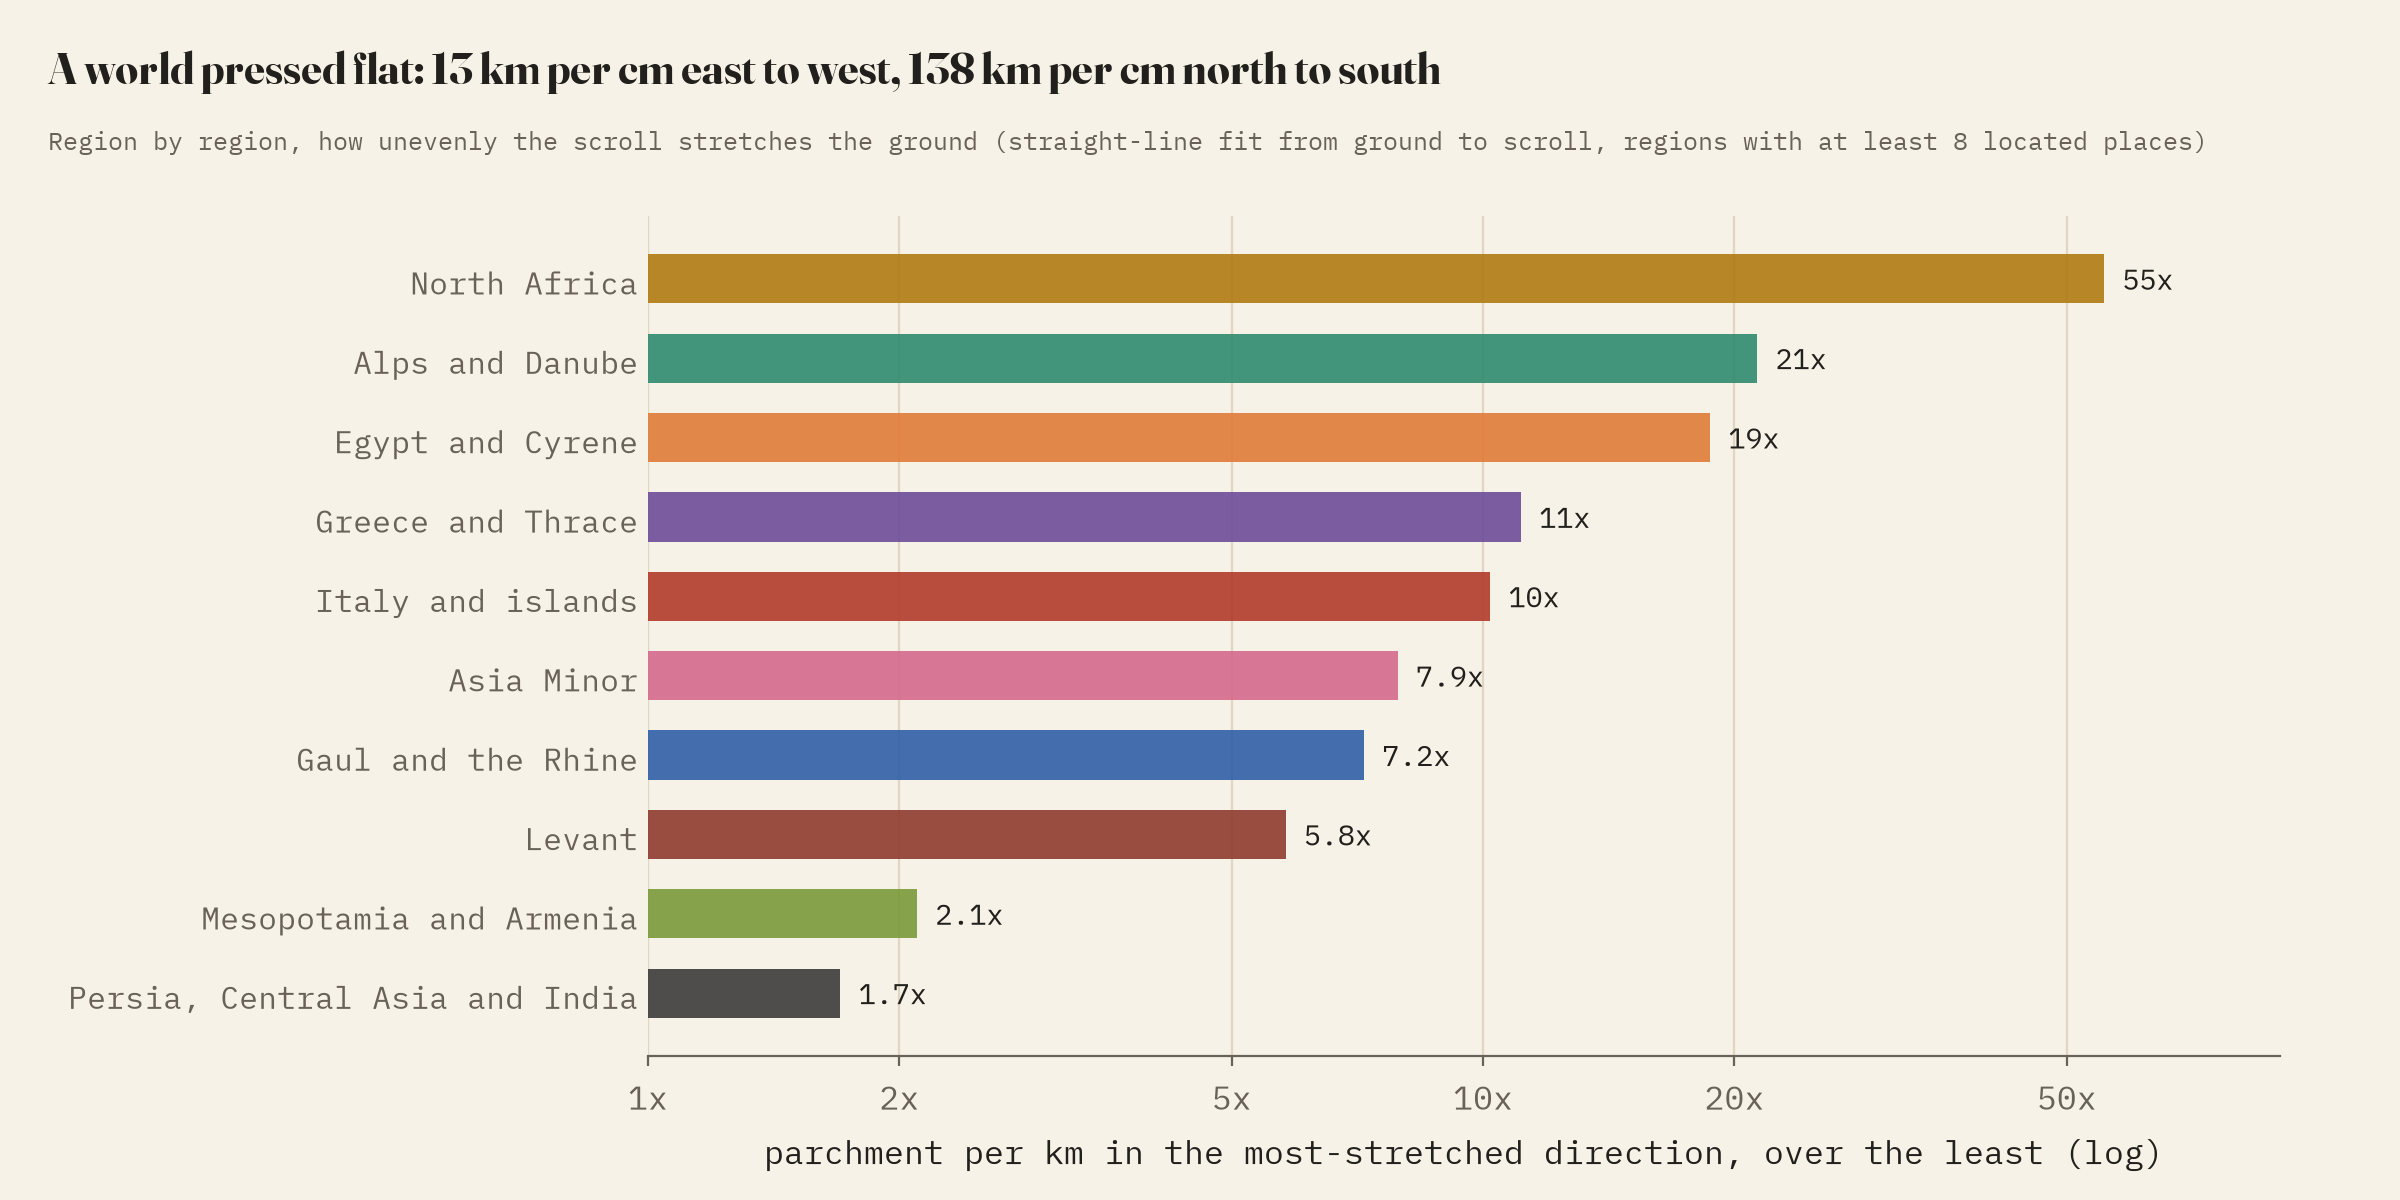
\includegraphics[width=\textwidth]{f_stretch.png}
\caption{Stretch by region: ratio of the largest to the smallest scale of an affine fit from ground to scroll.}\label{fig:stretch}\end{figure}
\begin{figure}[tbp]\centering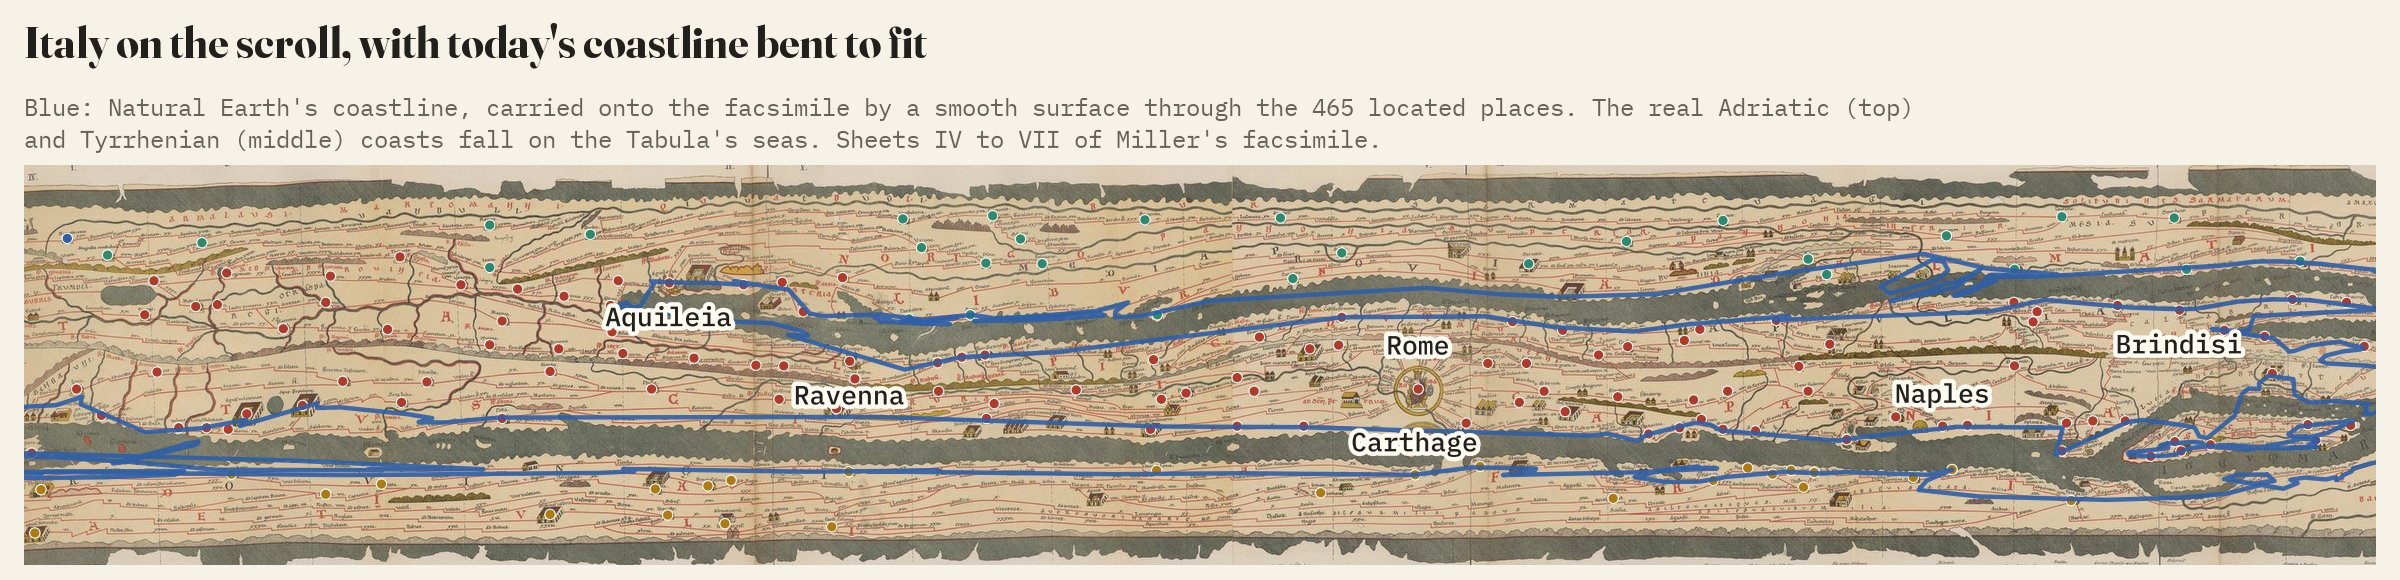
\includegraphics[width=\textwidth]{f_warp.jpg}
\caption{Italy on the scroll (sheets IV to VII) with the modern coastline carried onto it.}\label{fig:warp}\end{figure}
\begin{figure}[tbp]\centering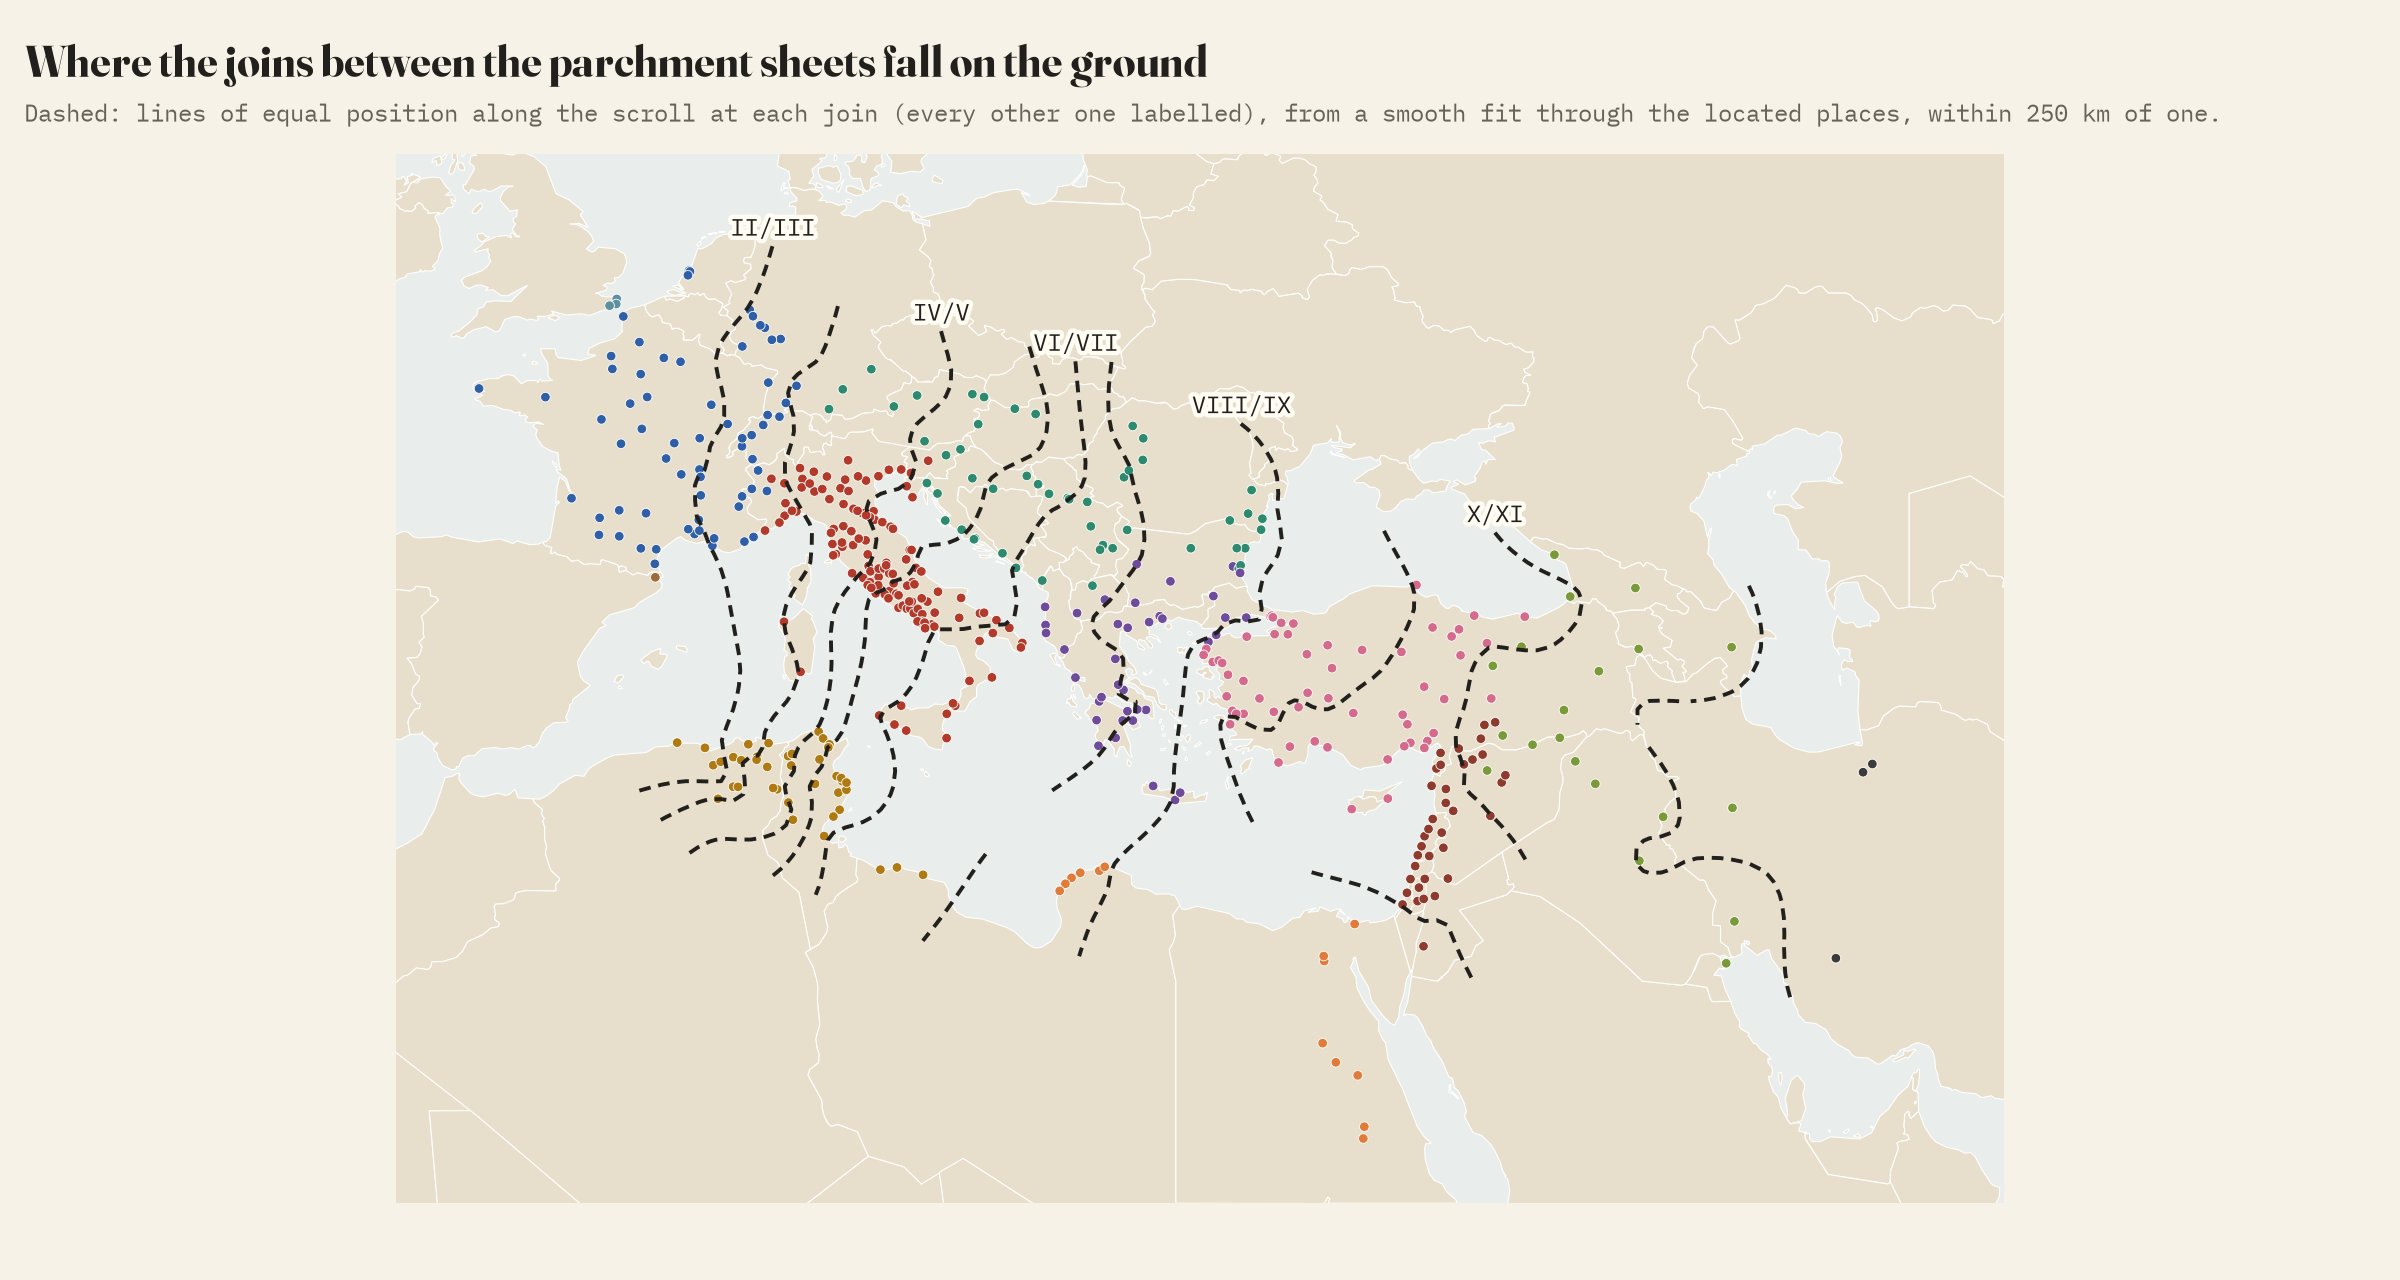
\includegraphics[width=\textwidth]{f_joins.png}
\caption{Where the joins between the surviving sheets fall on the ground.}\label{fig:joins}\end{figure}

\subsection{Space}
Italy and its islands take 17.3\% of the surviving scroll for 6.6\% of the land of the provinces, 2.62 times their share; Mesopotamia and Armenia 2.29, Greece and Thrace 1.55 and the Levant 1.34. Gaul (0.89), North Africa (0.82) and Asia Minor (0.99) receive about their share; Egypt (0.24) much less, though its province is mostly desert (Figure~\ref{fig:space}). Britain and Iberia are almost absent because their sheet is lost.

\begin{figure}[tbp]\centering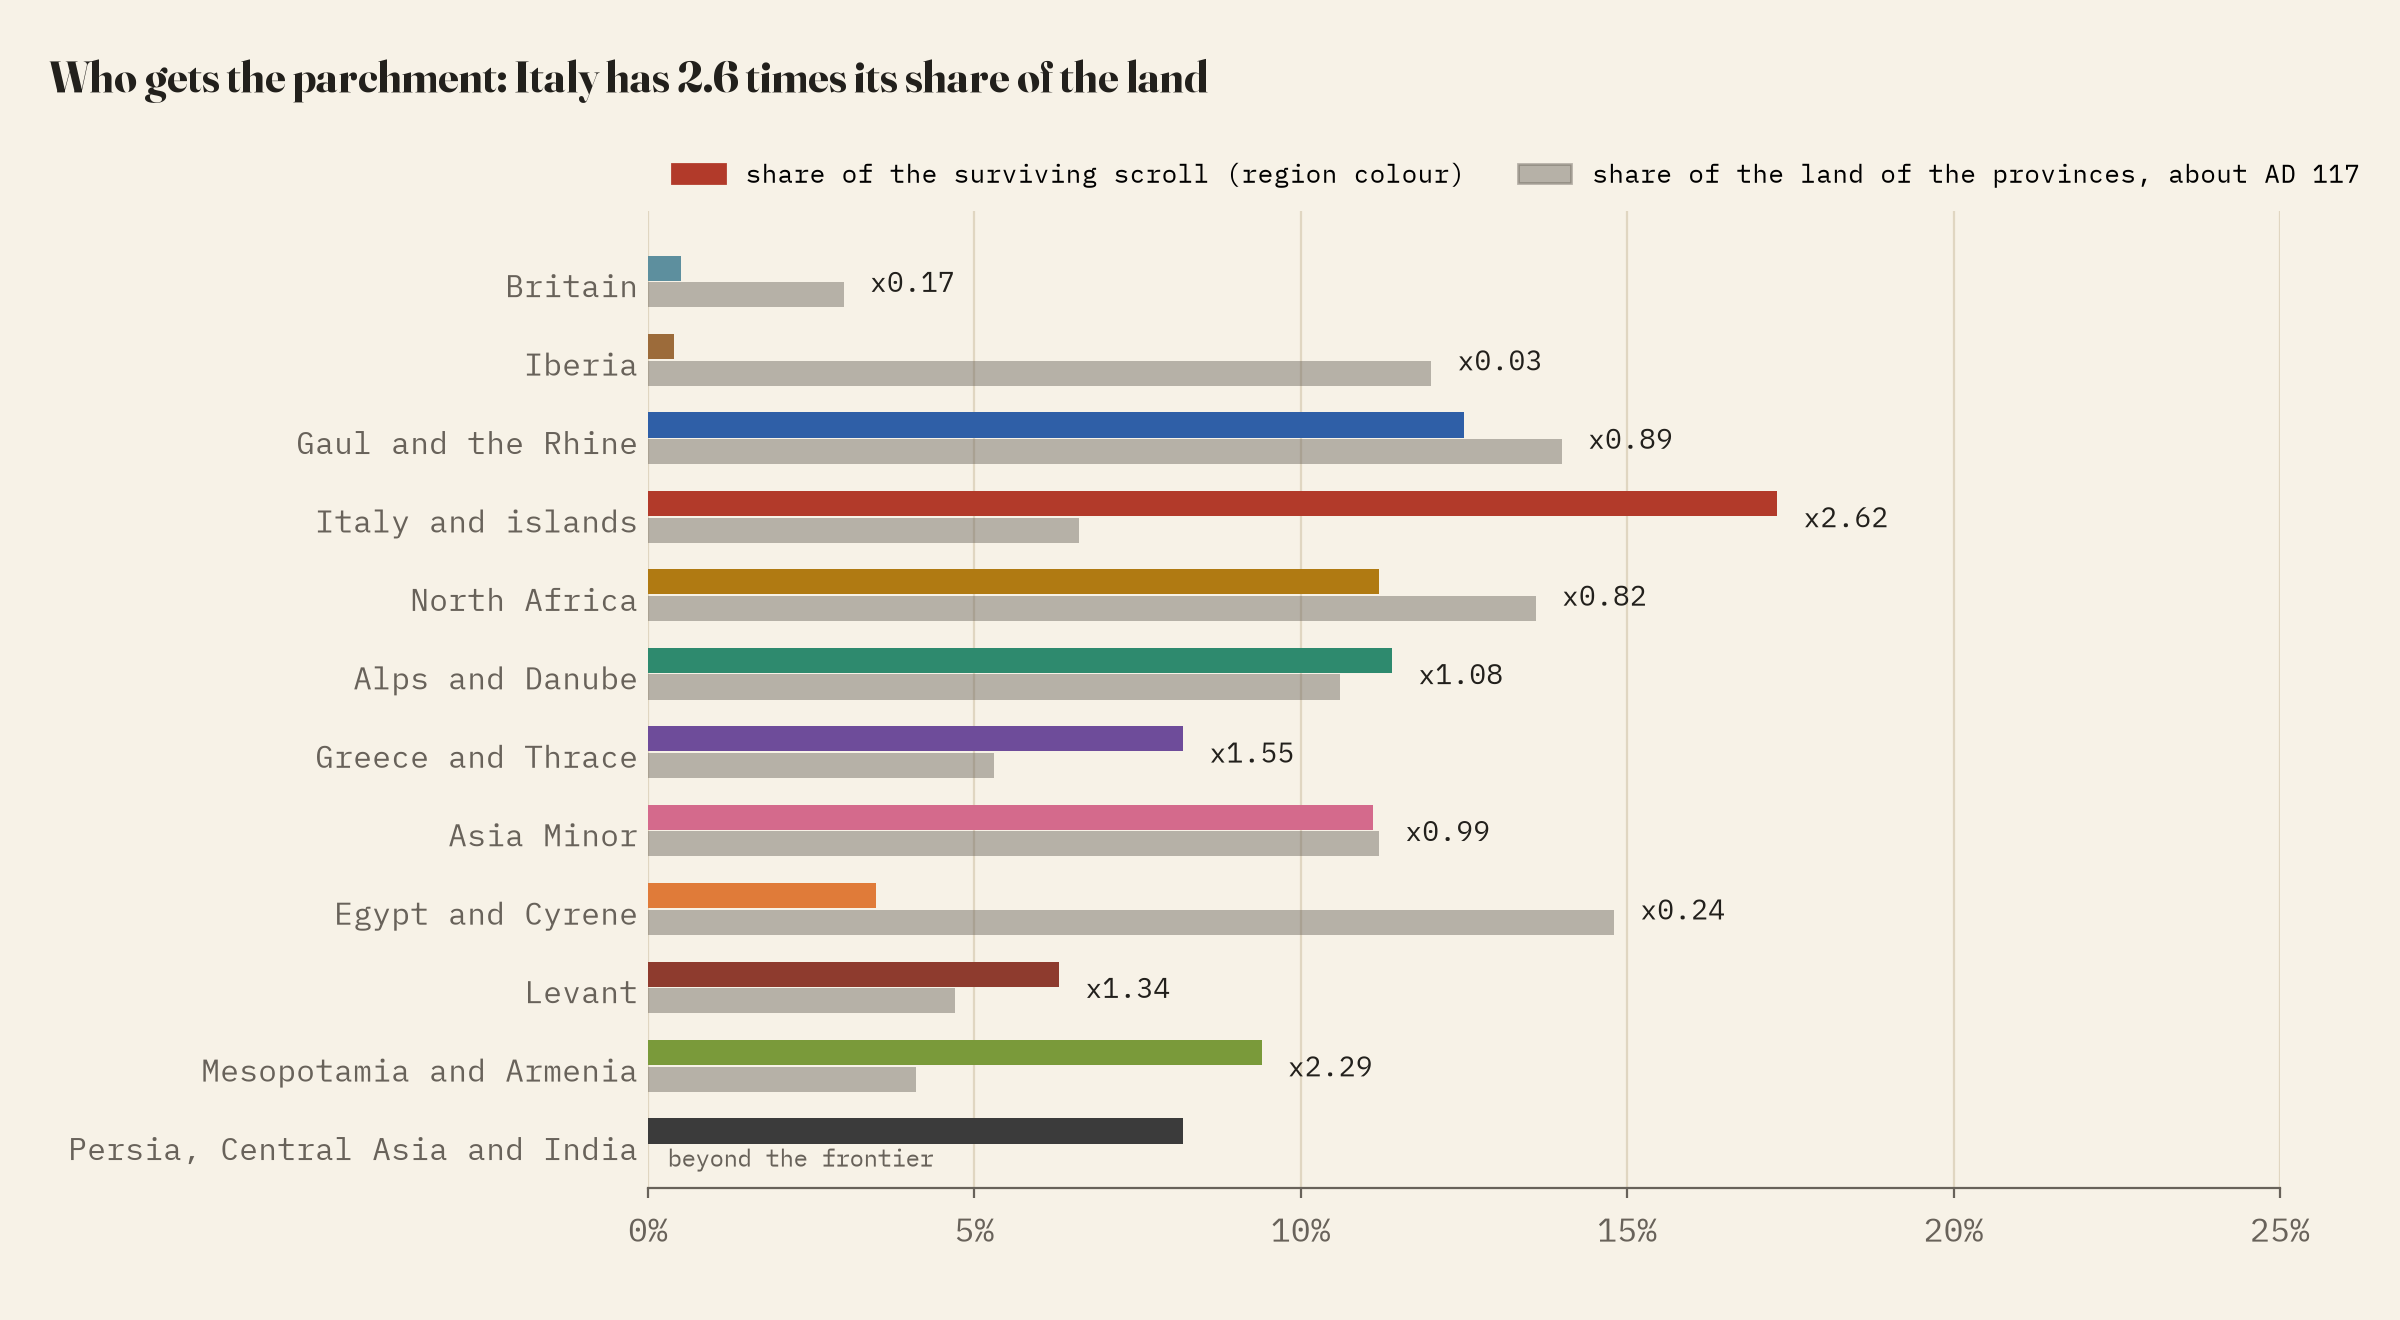
\includegraphics[width=\textwidth]{f_space.png}
\caption{Share of the surviving scroll against share of the land of the provinces of about AD 117.}\label{fig:space}\end{figure}

\begin{table}[tbp]\centering\footnotesize\caption{Regions: located places; share of the surviving scroll and of the land of the provinces (\%); ratio of the two; stretch; km per cm of parchment east-west and north-south from the regional fit; km of road written on the surviving sheets.}\label{tab:regions}\begin{tabular}{lrrrrrrrr}\toprule Region & Located & Scroll & Land & Ratio & Stretch & EW & NS & Road km\\\midrule
Britain & 3 & 0.5 & 3.0 & 0.17 &  &  &  & 367\\
Iberia & 1 & 0.4 & 12.0 & 0.03 &  &  &  & 81\\
Gaul and the Rhine & 65 & 12.5 & 14.0 & 0.89 & 7.2 & 7.7 & 43.9 & 12,781\\
Italy and islands & 129 & 17.3 & 6.6 & 2.62 & 10.2 & 4.4 & 8.6 & 9,044\\
North Africa & 39 & 11.2 & 13.6 & 0.82 & 55.4 & 2.5 & 22.5 & 7,169\\
Alps and Danube & 51 & 11.4 & 10.6 & 1.08 & 21.3 & 5.5 & 13.5 & 9,041\\
Greece and Thrace & 38 & 8.2 & 5.3 & 1.55 & 11.1 & 6.8 & 33.5 & 5,513\\
Asia Minor & 57 & 11.1 & 11.2 & 0.99 & 7.9 & 13.2 & 11.8 & 10,200\\
Egypt and Cyrene & 15 & 3.5 & 14.8 & 0.24 & 18.7 & 16.6 & 20.5 & 2,196\\
Levant & 36 & 6.3 & 4.7 & 1.34 & 5.8 & 8.5 & 12.4 & 4,914\\
Mesopotamia and Armenia & 20 & 9.4 & 4.1 & 2.29 & 2.1 & 23.8 & 37.1 & 5,051\\
Persia, Central Asia and India & 11 & 8.2 &  &  & 1.7 & 179.8 & 138.6 & 4,702\\
\bottomrule\end{tabular}\end{table}

\subsection{Rome}
Rome, one of three cities drawn as an enthroned figure with Constantinople and Antioch, and the start of 12 legs, lies 35.4\% of the way along the surviving strip, in Miller's sheet V; the middle of the strip falls near Skopje. With one lost sheet of median width Rome would lie at 40.7\%; it would be central with 3.3 lost sheets, and at 49.0\% with 3 (Figure~\ref{fig:rome}). If the map was designed with Rome at its centre, as some have argued \citep{talbert}, roughly three sheets, not one, are missing.

\begin{figure}[tbp]\centering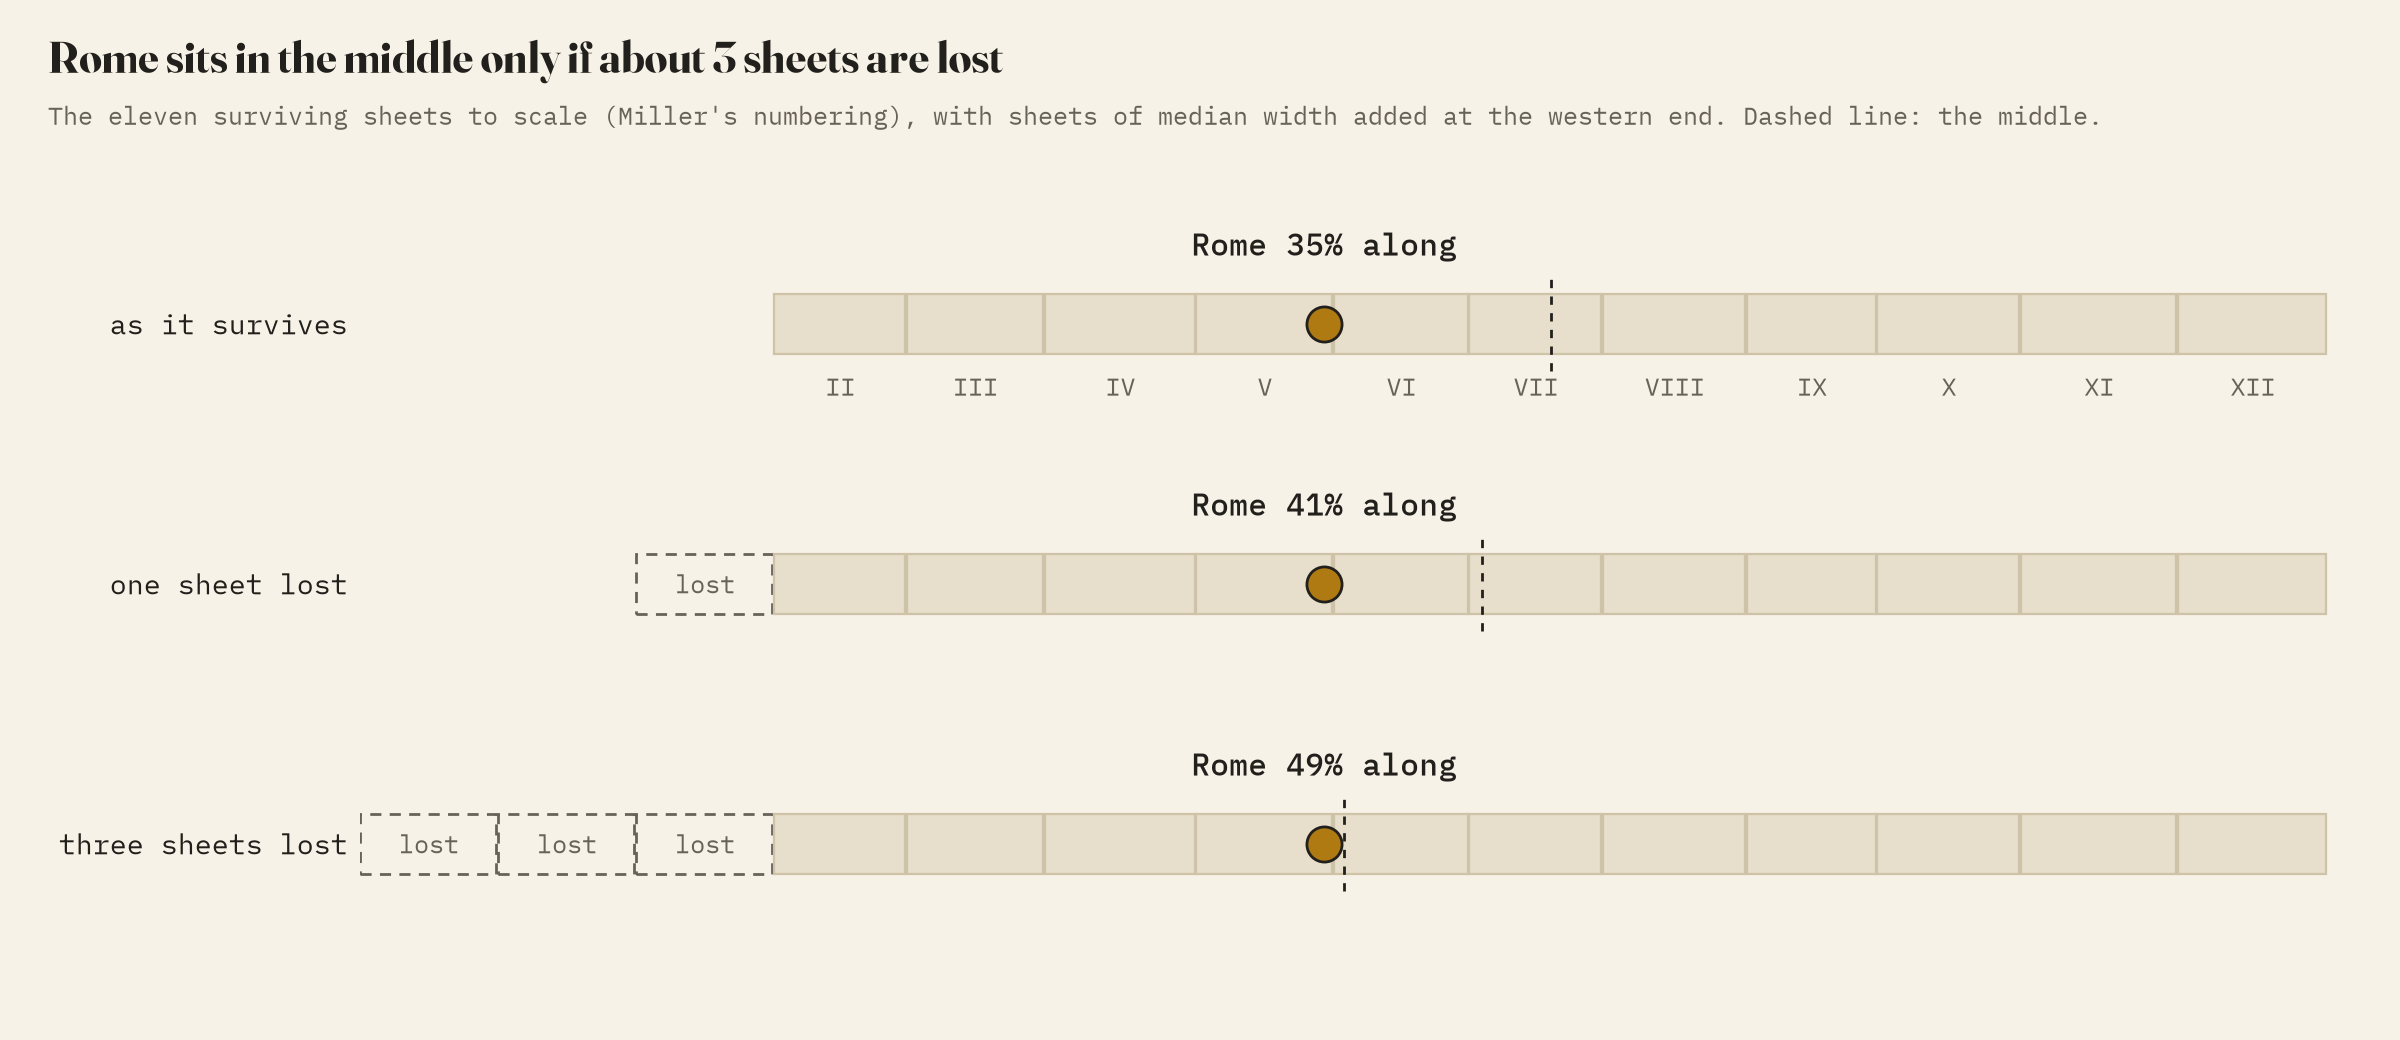
\includegraphics[width=\textwidth]{f_rome.png}
\caption{Rome's position along the strip as it survives and with one or three sheets added at the western end.}\label{fig:rome}\end{figure}

\subsection{Total road and days of travel}
The 2,720 surviving legs with a figure add up to 43,584 Roman miles, 4,598 leagues and 3,177 units in the far east, about 79,414 km (74,712 km without the far east), some 27\% of the length of the Itiner-e network. Walking it would take 3,530 days on foot, 1,765 by cart and 993 by courier relay. The reconstructed west adds 17,313 km; its legs behave like the Tabula's (median straight line 0.97 of the stated distance). From Rome, the map's figures give 92 days on foot to Constantinople, 156 to Jerusalem and 193 to Persepolis (Figure~\ref{fig:days}); with no sea routes, Carthage is 6,561 km away by land round the eastern Mediterranean.

\begin{figure}[tbp]\centering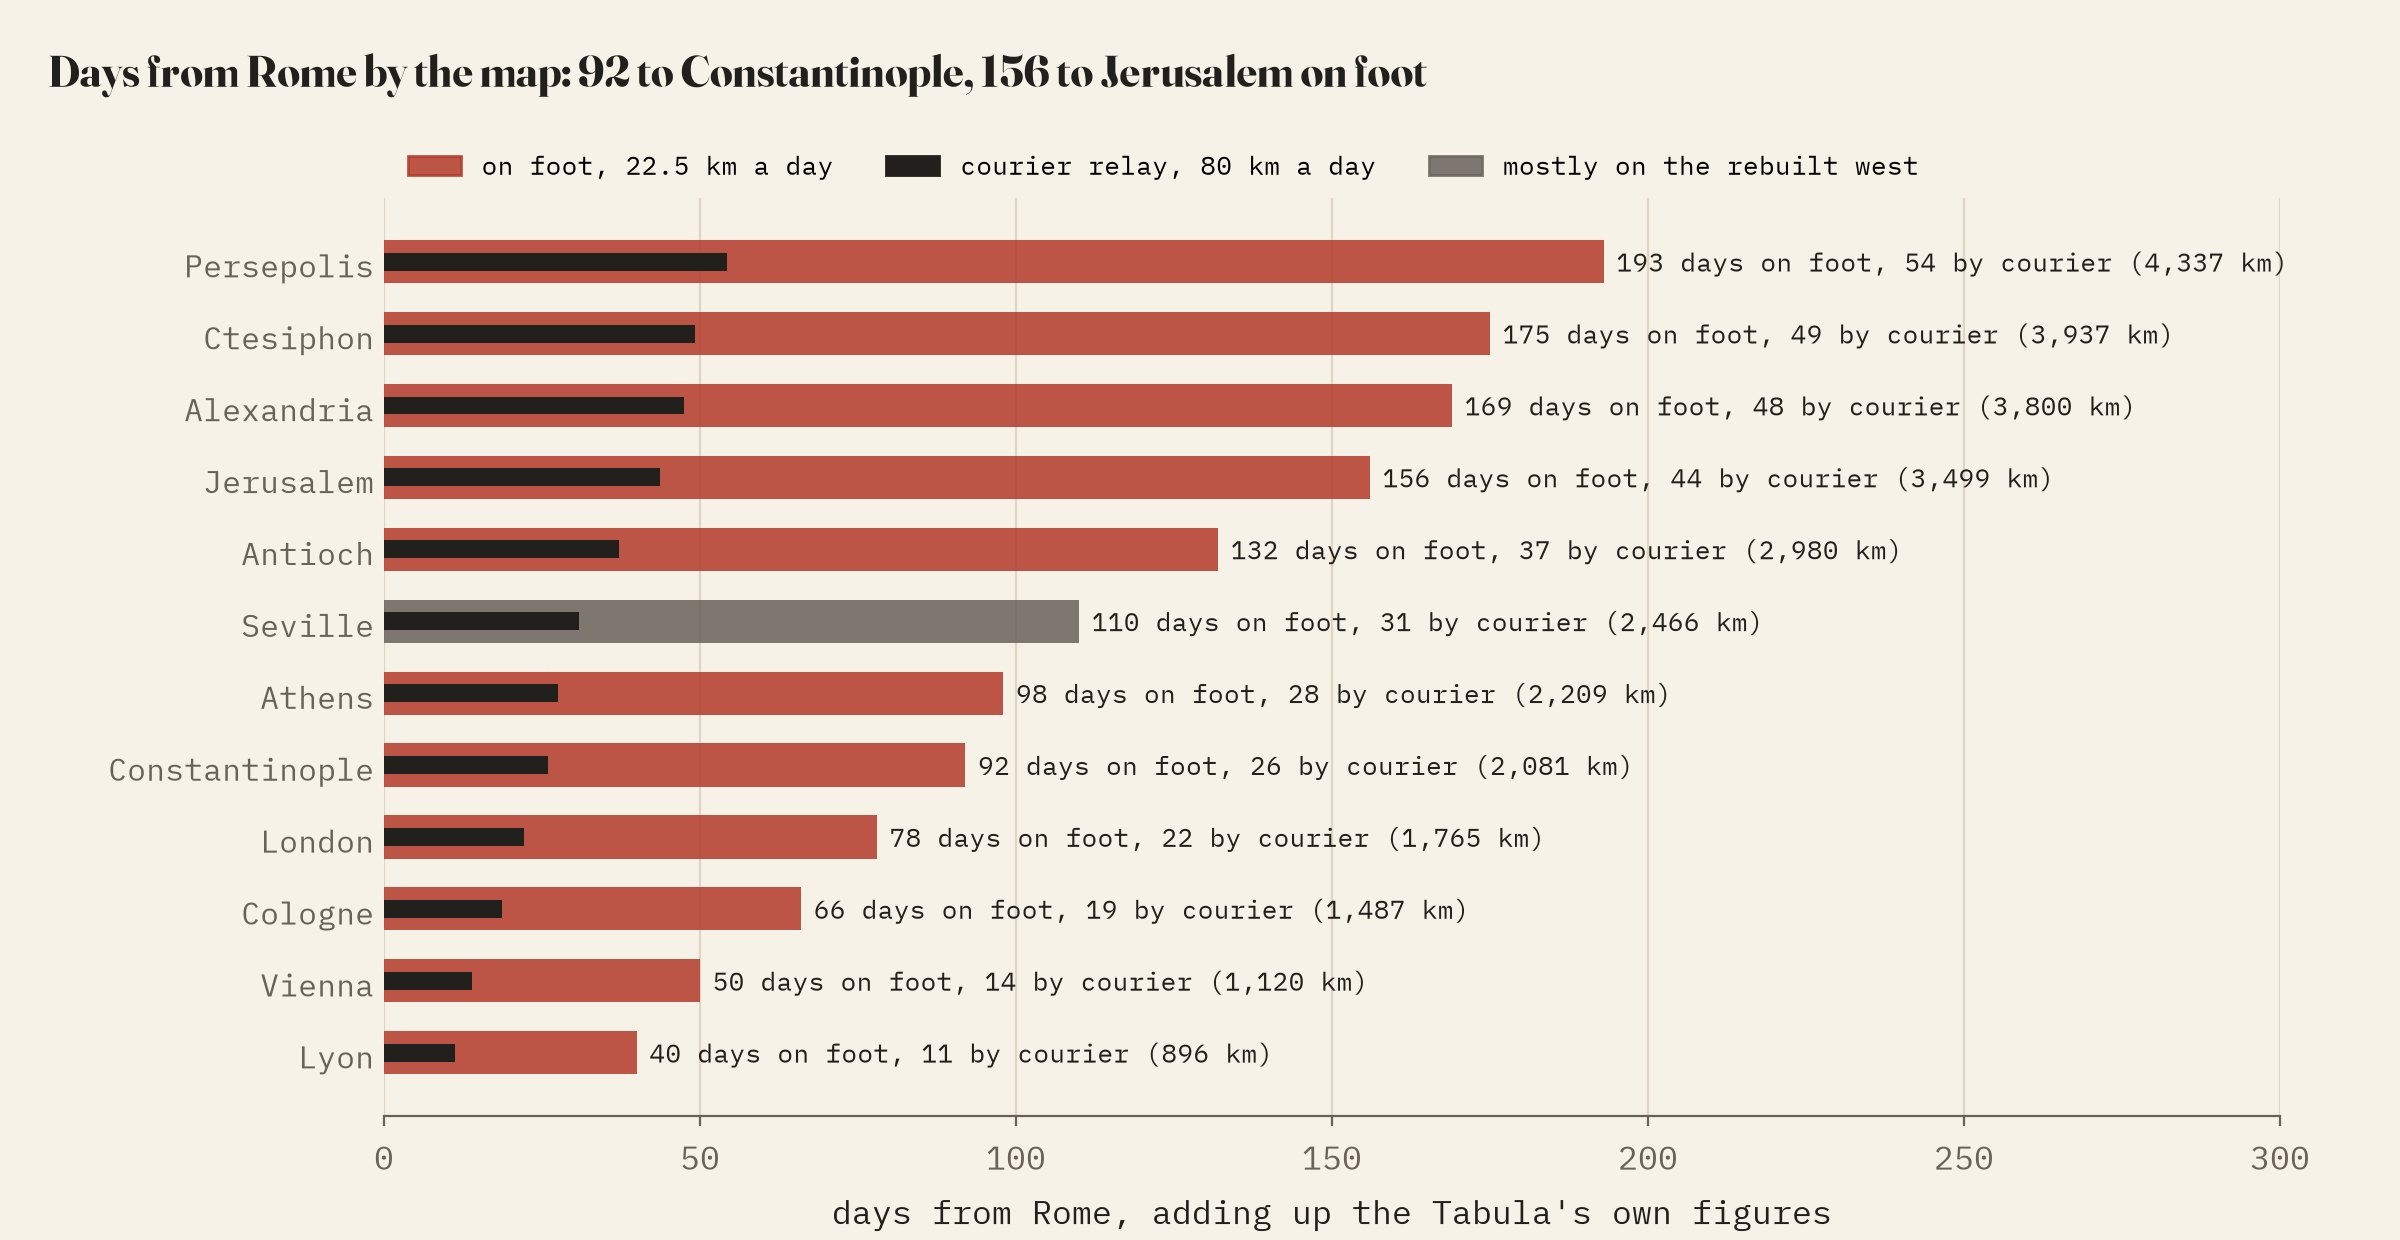
\includegraphics[width=\textwidth]{f_days.png}
\caption{Days of travel from Rome, adding the Tabula's own figures along the shortest route.}\label{fig:days}\end{figure}

\section{Limitations}
First, the coordinates and identifications are OmnesViae's and Talbert's, used as given; east of the Euphrates many are uncertain. Second, positions on the scroll were located by eye on a nineteenth-century facsimile, which is a careful copy but not the parchment; the sample favours legible places. Third, units are assigned by province, a simplification: the change from leagues to miles does not follow province boundaries exactly. Fourth, Itiner-e road lengths include every bend of the digitised road and the shortest path can detour round gaps, so road distances lean long. Fifth, the affine fits that measure stretch are rough, since nothing on this map is straight; the scroll shares depend on where I located places; and land shares count the desert of large provinces. Sixth, routes fill legs that have no figure with estimates, and ignore the sea.

\section{Conclusion}
The Peutinger Table gives up shape for length. It flattens the world by an order of magnitude north to south, turns whole regions on their sides, and spends its parchment on Italy and the East; but along its roads it keeps count. Its figures switch from miles to leagues where its own note says they should, sit where road distances should sit, and add up over long journeys to within a few per cent of the Roman roads mapped today. It is a diagram of the road network, drawn to be travelled rather than looked at.

\section*{Data and code availability}
The interactive comparison is at \url{https://maps.tristanhotham.com/peutinger/}. Data and code are at \url{https://github.com/Tristan-Hotham/peutinger} and archived with this paper at https://doi.org/10.5281/zenodo.23882605. Derived data are released under CC BY 4.0 and code under the MIT licence. The facsimile is public domain; OmnesViae data are credited to Ren\'e Voorburg and Richard Talbert (no licence stated, used as factual data); Itiner-e is CC BY 4.0; DARE is CC BY-SA; Pleiades CC BY 3.0.

\section*{AI statement}
I wrote the text, with drafting and editing assistance from Claude (Anthropic), which also helped prepare the analysis code. I reviewed and checked all text and results.

\begin{thebibliography}{9}
\bibitem[Talbert(2010)]{talbert} Talbert, R. J. A. (2010) \textit{Rome's World: the Peutinger Map Reconsidered}. Cambridge: Cambridge University Press.
\bibitem[Voorburg(2026)]{omnesviae} Voorburg, R. (2026) OmnesViae: Roman routeplanner, based on the Peutinger map. \url{https://omnesviae.org/}
\bibitem[Miller(1887)]{miller} Miller, K. (1887) \textit{Castori Romanorum cosmographi tabula quae dicitur Peutingeriana}. Ravensburg. Facsimile, Wikimedia Commons, public domain. \url{https://commons.wikimedia.org/wiki/File:TabulaPeutingeriana.jpg}
\bibitem[de Soto et al.(2025)]{itinere} de Soto, P., Pa\v{z}out, A., Brughmans, T. et al. (2025) Itiner-e: the digital atlas of ancient roads. Zenodo, \url{https://doi.org/10.5281/zenodo.17122148}. CC BY 4.0.
\bibitem[Hotham(2026)]{romanroads} Hotham, T. (2026) Roads of the Roman Empire. \url{https://maps.tristanhotham.com/roman-roads/}
\bibitem[{\AA}hlfeldt(2026)]{dare} {\AA}hlfeldt, J. (2026) Digital Atlas of the Roman Empire (DARE), provinces. CC BY-SA.
\bibitem[Pleiades(2026)]{pleiades} Bagnall, R. et al., eds. (2026) Pleiades: a gazetteer of past places, version 4.1. CC BY 3.0. \url{https://pleiades.stoa.org/}
\bibitem[Natural Earth(2026)]{naturalearth} Natural Earth (2026) Admin 0 countries and land, 1:50m. Public domain. \url{https://www.naturalearthdata.com/}
\bibitem[Wikipedia(2026)]{wiki} Wikipedia contributors (2026) Roman roads (revision 1383149720). CC BY-SA 4.0. \url{https://en.wikipedia.org/wiki/Roman_roads}
\end{thebibliography}

\clearpage
\appendix
\section{The located places}
{\footnotesize\setlength{\tabcolsep}{4pt}\begin{longtable}{p{4.6cm}p{5.2cm}lrrl}\caption{The 465 places located on Miller's facsimile, west to east: name as written (OmnesViae), modern place, sheet, position in facsimile pixels and confidence.}\label{tab:located}\\\toprule Name on the map & Today & Sheet & x & y & Read\\\midrule\endfirsthead\toprule Name on the map & Today & Sheet & x & y & Read\\\midrule\endhead
Burdegalo & Bordeaux & II & 520 & 940 & high\\
Eliberre & Auch & II & 580 & 1,030 & medium\\
Lemavio & Lympne & II & 615 & 765 & medium\\
Ratvpis & Richborough & II & 622 & 635 & high\\
Dvbris & Dover & II & 628 & 700 & high\\
Ivncaria &  & II & 800 & 1,125 & high\\
Tolosa & Toulouse & II & 825 & 1,070 & high\\
Gesocribate & Brest & II & 855 & 836 & high\\
Lvgdvno & Katwijk aan Zee & II & 885 & 590 & high\\
Gesogiaco qvod nvnc Bononia & Boulogne-sur-Mer & II & 885 & 665 & high\\
Foro Adriani & Voorburg & II & 960 & 600 & high\\
Pretoriv̄ Agrippine & Valkenburg & II & 1,000 & 575 & high\\
Aginnvm & Agen & II & 1,020 & 1,030 & high\\
Rvsvccvrv colon̄ & Dellys | Tigzirt & II & 1,040 & 1,295 & high\\
Condate & Rennes & II & 1,085 & 825 & medium\\
Carcassione & Casrcassonne & II & 1,205 & 1,095 & high\\
Bibona & Cahors & II & 1,225 & 1,035 & high\\
Ratvmagvs & Rouen & II & 1,330 & 682 & high\\
Mediolano avtercorvm & Evreux & II & 1,355 & 740 & high\\
Sammarobriva & Amiens & II & 1,430 & 620 & high\\
Sitifi col. & Sétif & II & 1,470 & 1,435 & high\\
Rvscione & Château Roussillon & II & 1,530 & 1,180 & high\\
Segodvni & Rodez & II & 1,540 & 1,090 & high\\
Argantomago & Saint-Marcel & II & 1,555 & 955 & medium\\
Casarodvno & Tours & II & 1,580 & 815 & high\\
Narbone & Narbonne & II & 1,672 & 1,185 & high\\
Cenabo & Orléans & II & 1,730 & 788 & high\\
Avaricvm & Bourges & II & 1,783 & 877 & high\\
Lvteci & Paris & II & 1,790 & 735 & high\\
Avg Svessorvm & Soissons & II & 1,820 & 660 & high\\
Aqvis Calidis & Vichy & II & 1,880 & 1,035 & high\\
Aqvis Segeste & Sceaux-du-Gâtinais & II & 1,890 & 805 & high\\
Cvlchvl Colonia & Djémila & II & 1,995 & 1,358 & high\\
AQVIS BORMONIS & Bourbon-Lancy & II & 2,040 & 980 & high\\
Saldas Colonia & Béjaïa & II & 2,055 & 1,298 & high\\
Nemvso & Nîmes & II & 2,190 & 1,148 & high\\
Dvrocortoro & Reims & II & 2,235 & 693 & high\\
Aqvis Segete & Moingt & II & 2,280 & 1,080 & medium\\
Andemantvnno & Langres & II & 2,305 & 738 & high\\
Arelato & Arles & II & 2,415 & 1,125 & high\\
Cabillione & Chalons-sur-Saóne & II & 2,440 & 845 & high\\
Lvgdvno capvt Galliarvm & Lyon & II & 2,485 & 915 & medium\\
Clano & Saint-Rémy-de-Provence & II & 2,515 & 1,115 & medium\\
Arvsione & Orange & III & 2,665 & 1,020 & high\\
Agripina & Köln & III & 2,675 & 520 & high\\
Masilia Grecorvm & Marseille & III & 2,683 & 1,168 & high\\
Vigenna & Vienne & III & 2,685 & 980 & high\\
Vesontine & Besançon & III & 2,730 & 762 & high\\
Valentia & Valence & III & 2,755 & 1,012 & high\\
Bonnae & Bonn & III & 2,772 & 525 & high\\
Aquis Sestis & Aix-en Provence & III & 2,792 & 1,158 & high\\
Antvnnaco & Andernach & III & 2,970 & 512 & high\\
Avg Tresvirorvm & Trier & III & 3,010 & 622 & high\\
Ebvrodvno & Yverdon-les-Bains & III & 3,040 & 768 & high\\
Conflventes & Koblenz & III & 3,080 & 495 & high\\
Aventicvm Heletiorvm & Avenches & III & 3,282 & 780 & high\\
Lambese &  & III & 3,305 & 1,455 & high\\
Foro ivlii & Fréjus & III & 3,310 & 1,175 & high\\
Lacvm Losonne & Lausanne & III & 3,380 & 825 & high\\
Bingiv̄ & Bingen & III & 3,400 & 512 & high\\
Mogontiaco & Mainz & III & 3,472 & 522 & high\\
Ebvrvno & Embrun & III & 3,480 & 1,000 & high\\
Antipoli & Antibes & III & 3,500 & 1,180 & high\\
Brigantione & Briançon & III & 3,580 & 1,000 & high\\
Rvsicade Colonia & Skikda & III & 3,718 & 1,295 & high\\
Milev Colonia & Mila & III & 3,782 & 1,348 & high\\
Albentimillo & Ventimiglia & III & 3,835 & 1,112 & high\\
Octodvro & Martigny & III & 3,900 & 755 & high\\
Salodvrvm & Solothurn & III & 3,970 & 675 & high\\
Albingavno & Albenga & III & 4,030 & 1,112 & high\\
Thamvgadi & Timgad & III & 4,035 & 1,460 & high\\
Argentorate & Strasbourg & III & 4,065 & 568 & high\\
Vadis Sabates & Vado Ligure & III & 4,175 & 1,130 & high\\
Segvsione & Susa & III & 4,200 & 922 & high\\
Avgvsta Pretoria & Aosta & III & 4,395 & 822 & high\\
Aqvis Tatelis & Acqui Terme & III & 4,470 & 1,062 & high\\
Avgvsta Rvracvm & Augst & III & 4,480 & 618 & high\\
Hasta &  & III & 4,500 & 1,130 & medium\\
Vindonissa & Windisch & III & 4,548 & 602 & high\\
Avgvsta Tavrinorvm & Torino & III & 4,620 & 857 & high\\
Cirta Colonia & Constantine & III & 4,625 & 1,342 & high\\
Genva & Genova & III & 4,655 & 1,100 & high\\
Eporedia & Ivrea & III & 4,665 & 725 & high\\
Brigobanne & Hüfingen & III & 4,805 & 562 & high\\
Vergellis & Vercelli & III & 4,815 & 720 & high\\
Tvrribvs &  & IV & 4,948 & 1,220 & high\\
Caralis &  & IV & 5,025 & 1,212 & high\\
Ad aqvas Hercvlis & Hammam Sidi el Hadj & IV & 5,035 & 1,470 & high\\
Aqvis Thibilitanis & Hammam Meskoutine & IV & 5,055 & 1,330 & high\\
Samvlocenis & Rottenburg am Neckar & IV & 5,140 & 518 & high\\
Lvca & Lucca & IV & 5,170 & 1,005 & high\\
Pisis & Pisa & IV & 5,250 & 1,090 & high\\
Avgvsta vindelicv̄ & Augsburg & IV & 5,270 & 572 & high\\
Ticeno & Pavia & IV & 5,390 & 765 & high\\
Como & Como & IV & 5,420 & 655 & high\\
Pistoris & Pistoia & IV & 5,430 & 950 & high\\
Velinis & Volterra & IV & 5,500 & 1,130 & high\\
Mediolanvm & Milano & IV & 5,555 & 738 & high\\
Cambodvno & Kempten & IV & 5,575 & 532 & high\\
Vadis Volateris & Vada \textasciitilde{} Rosignano Marittimo & IV & 5,590 & 1,130 & high\\
Lavde pompeia & Lodi & IV & 5,625 & 732 & high\\
Bergomvm & Bergamo & IV & 5,655 & 630 & high\\
Popvlonio & Populonia & IV & 5,660 & 1,135 & high\\
Hyppone Regio & Annaba & IV & 5,670 & 1,280 & high\\
Aqvas volaternas & Terme di Pomarance & IV & 5,720 & 1,085 & high\\
Placentia & Piacenza & IV & 5,838 & 810 & high\\
Aqvae Popvlaniae & Venturina-Terme & IV & 5,900 & 1,058 & high\\
Cremona & Cremone & IV & 5,975 & 725 & high\\
Thibili & Announa & IV & 5,975 & 1,345 & high\\
Brixia & Brescia & IV & 5,990 & 640 & high\\
Florentia Tvscorvm & Firenze & IV & 6,030 & 980 & high\\
Tipasa & Tabet es-Sefra & IV & 6,155 & 1,312 & medium\\
Parna & Parma & IV & 6,175 & 812 & high\\
Tredente & Trento & IV & 6,215 & 578 & high\\
Sena Ivlia & Siena & IV & 6,220 & 1,048 & high\\
Bitvriza & Montevarchi & IV & 6,302 & 982 & medium\\
Verona & Verona & IV & 6,412 & 668 & high\\
Regino & Regensburg & IV & 6,505 & 475 & high\\
Ivavo & Salzburg & IV & 6,505 & 612 & high\\
Mvtina & Modena & IV & 6,505 & 862 & high\\
Cosa & Ansedonia & IV & 6,545 & 1,100 & high\\
Mantva & Mantova & IV & 6,545 & 785 & high\\
Vicētia &  & IV & 6,595 & 682 & high\\
Adretio & Arezzo & IV & 6,700 & 948 & high\\
Ad Aqvas casaris & Youks \textasciitilde{} Tebessa & IV & 6,700 & 1,410 & high\\
Bononia & Bologna & IV & 6,728 & 875 & high\\
Patavis & Podova & IV & 6,745 & 705 & high\\
Ovilia & Wels & IV & 6,830 & 505 & high\\
Altino & Altino & IV & 6,895 & 735 & high\\
Hostilia & Ostiglia & IV & 6,900 & 820 & high\\
Concordia & Concordia Sagittaria & IV & 6,920 & 655 & high\\
Claterna & Osteria Grande & IV & 6,935 & 890 & high\\
Clvsio & Chiusi & IV & 7,028 & 1,005 & high\\
Sicca Vēria & El Kef & IV & 7,040 & 1,328 & high\\
Theveste & Tebessa & IV & 7,080 & 1,412 & high\\
Aqvileia & Aquileia & IV & 7,085 & 662 & high\\
Foro corneli & Imola & IV & 7,165 & 905 & high\\
Simitv Colonia & Chemtou & IV & 7,210 & 1,318 & high\\
Theleote col. & Medinet el Kedima & IV & 7,265 & 1,440 & medium\\
Bvlla Regia &  & IV & 7,285 & 1,300 & high\\
Tergeste & Trieste & IV & 7,325 & 668 & high\\
Faventia & Faenza & IV & 7,365 & 928 & high\\
Volsinis & Bolsena & V & 7,440 & 1,038 & high\\
Parentio & Poreč & V & 7,450 & 660 & high\\
Foro Livi & Forlì & V & 7,455 & 930 & high\\
Pola & Pula & V & 7,518 & 755 & high\\
Capsa Colonia & Gafsa & V & 7,610 & 1,450 & high\\
Aqvas Passaras & Bagni Giasinelli & V & 7,625 & 1,068 & high\\
Emona & Ljubljana & V & 7,645 & 645 & high\\
Ipponte diarito & Bizerta & V & 7,665 & 1,272 & high\\
Ravenna & Ravenna & V & 7,668 & 915 & high\\
Cvrita cesena & Cesena & V & 7,685 & 972 & high\\
Vindobona & Wien & V & 7,840 & 455 & high\\
Tarsatica & Rijeka Trsat & V & 7,860 & 778 & high\\
Virvno & Maria Saal & V & 7,900 & 548 & high\\
ARIMINO & Rimini & V & 7,952 & 920 & high\\
Ameria & Amelia & V & 7,955 & 1,012 & high\\
Pisavro & Pésaro & V & 8,030 & 902 & high\\
Senia & Senj & V & 8,058 & 765 & high\\
Fano Fvrtvnae & Fano & V & 8,105 & 895 & high\\
Celeia & Celje & V & 8,108 & 598 & high\\
Tarqvinis & Tarquinia & V & 8,110 & 1,100 & high\\
Carnvnto & Deutsch Altenburg & V & 8,130 & 445 & high\\
Foro clodo &  & V & 8,135 & 1,052 & high\\
Sabarie & Szombathely & V & 8,220 & 520 & high\\
Petavione & Ptuj & V & 8,290 & 600 & high\\
Faleros & Civita Castellana & V & 8,400 & 1,008 & high\\
Brigantio & Szõny \textasciitilde{} Komárom & V & 8,622 & 458 & high\\
Aqvas Apollinaris & Bagni di Stigliano & V & 8,640 & 1,135 & high\\
Asclopiceno & Ascoli Piceno & V & 8,650 & 910 & high\\
Vtica Colonia & Bou Shater \textasciitilde{} Tunis & V & 8,660 & 1,268 & high\\
Iadera & Zadar & V & 8,662 & 765 & high\\
Spoletio & Spoleto & V & 8,675 & 1,038 & high\\
Fano Fvgitivi & Monte Somma \textasciitilde{} Spoleto & V & 8,755 & 1,018 & high\\
Pyrgos & \textasciitilde{} Santa Severa & V & 8,920 & 1,125 & high\\
Interamnio & Terni & V & 8,920 & 968 & high\\
Veios & Veio \textasciitilde{} Isola Farnese & V & 8,975 & 1,012 & high\\
Firmoviceno & Fermo & V & 8,992 & 837 & high\\
Aqvinco & Budapest & V & 9,060 & 452 & high\\
Sardona & Skradin & V & 9,100 & 648 & high\\
Alsivm & Palo \textasciitilde{} Ladispoli & V & 9,135 & 1,125 & high\\
Aqve cvtillie & Paterno \textasciitilde{} Cittaducale & V & 9,155 & 875 & high\\
Tvbvrbomaivs & \textasciitilde{} El Fahs & V & 9,190 & 1,340 & high\\
Reate & Rieti & V & 9,248 & 863 & high\\
Siscia & Sisak & V & 9,258 & 565 & high\\
Castello Firmani & Santa Maria a Mare & V & 9,258 & 773 & high\\
Chartagine Colon̄ & Tunis & V & 9,495 & 1,282 & high\\
ROMA & Roma & V & 9,505 & 1,005 & high\\
Hostis & Ostia & VI & 9,660 & 1,115 & high\\
Maxvla & Radès & VI & 9,705 & 1,255 & high\\
Preneste & Palestrina & VI & 9,730 & 922 & high\\
Hadria & Atri & VI & 9,810 & 787 & high\\
Aricia & Ariccia & VI & 9,832 & 1,048 & high\\
Carsvlis & Civita Seconda & VI & 9,855 & 922 & medium\\
Servttio & Bosanska Gradiška & VI & 9,862 & 600 & high\\
Conpito Anagnino & Anagni & VI & 9,912 & 1,012 & high\\
Ostia Eterni & Pescara & VI & 9,972 & 815 & high\\
Tres Tabernas & \textasciitilde{} Cisterna di Latina & VI & 9,980 & 1,078 & high\\
Marrvbio & San Benedetto dei Marsi & VI & 10,088 & 895 & high\\
Aqvas Regias &  & VI & 10,135 & 1,358 & high\\
Ferentinvm & Ferentino & VI & 10,150 & 1,030 & high\\
Mvrsa maior & Osijek & VI & 10,178 & 528 & high\\
Corfinio & Corfinio & VI & 10,182 & 868 & high\\
Terracina & Terracina & VI & 10,250 & 1,150 & high\\
Fvndis & Fondi & VI & 10,350 & 1,130 & high\\
Svlmone & Sulmona & VI & 10,365 & 848 & high\\
Aqvino & Aquino & VI & 10,395 & 1,040 & high\\
Larinv̄ & Larino & VI & 10,415 & 812 & high\\
Formis & Formia & VI & 10,420 & 1,103 & high\\
Hadrito & Soûsse & VI & 10,458 & 1,300 & high\\
Cornaco & Sotin & VI & 10,490 & 460 & high\\
Mentvrnis & Minturno & VI & 10,490 & 1,135 & high\\
Casinvm & Montecassino & VI & 10,505 & 1,012 & high\\
Rvspina &  & VI & 10,570 & 1,260 & high\\
Sinvessa & \textasciitilde{} Mondragone & VI & 10,595 & 1,140 & high\\
Lepteminvs & Lamta & VI & 10,650 & 1,280 & high\\
Siponto & Siponto \textasciitilde{} Manfredonia & VI & 10,662 & 783 & high\\
Tapsvm & Rass Dimasse & VI & 10,710 & 1,268 & high\\
Esernie & Isernia & VI & 10,735 & 932 & high\\
Thisdro Col. & El Djem & VI & 10,750 & 1,322 & high\\
Teano Scedicino & Teano & VI & 10,765 & 1,012 & high\\
Salona & Solin & VI & 10,765 & 585 & high\\
Svllecti & Rass Salakta & VI & 10,785 & 1,275 & high\\
Spalato & Split & VI & 10,825 & 635 & high\\
Bobiano & Bojano & VI & 10,835 & 860 & high\\
Cvmas & Cuma & VI & 10,890 & 1,168 & high\\
Pvteolis & Pozzuoli & VI & 11,048 & 1,095 & high\\
Capvae & Santa Maria Capua Vetere & VI & 11,062 & 1,045 & high\\
Taparvra & Sfax & VI & 11,105 & 1,290 & high\\
Neapoli & Napoli & VI & 11,200 & 1,125 & high\\
Sirmivm & Sremska Mitrovica & VI & 11,212 & 510 & high\\
Macomades Minores &  & VI & 11,230 & 1,265 & high\\
Herclanivm & Ercolano & VI & 11,280 & 1,122 & high\\
Barivm & Bari & VI & 11,430 & 725 & high\\
Narona & Vid \textasciitilde{} Metković & VI & 11,432 & 618 & high\\
Benebento & Benevento & VI & 11,432 & 930 & high\\
Venvsie & Venosa & VI & 11,492 & 788 & high\\
Bvtvntos & Bitonto & VI & 11,505 & 755 & high\\
Svrrento & Sorrento & VI & 11,585 & 1,205 & high\\
Tavrvno & Zemun & VI & 11,585 & 448 & high\\
Pompeis & Pompei & VI & 11,600 & 1,115 & high\\
Tacape col. & Gabès & VI & 11,615 & 1,365 & high\\
Nvceria & Nocera & VI & 11,685 & 1,108 & high\\
Gnatie & Torre Egnazia \textasciitilde{} Fasano & VI & 11,765 & 735 & high\\
Salerno &  & VI & 11,790 & 1,108 & high\\
Lilybeo & Marsala & VI & 11,872 & 1,222 & high\\
Singidvno & Beograd & VII & 11,948 & 452 & high\\
Panormo & Palermo & VII & 11,950 & 1,175 & medium\\
Brindisi &  & VII & 11,965 & 750 & high\\
Aqvas labodes & Sciacca & VII & 11,970 & 1,205 & high\\
Epitavro & Cavtat & VII & 11,988 & 618 & high\\
Agrigento & Agrigento & VII & 12,065 & 1,185 & high\\
Tarento & Taranto & VII & 12,110 & 815 & high\\
Heraclea & Policoro & VII & 12,240 & 835 & high\\
Aqve Ange & Bagni di Sant'Eufemia & VII & 12,265 & 955 & high\\
Ydrvnte & Otranto & VII & 12,330 & 715 & high\\
Scobre & Shkodër & VII & 12,355 & 592 & high\\
Tavromenio &  & VII & 12,380 & 1,120 & high\\
Siracvsis & Siracusa & VII & 12,405 & 1,170 & medium\\
Castra Minervae & Castro & VII & 12,505 & 725 & high\\
Messana & Messina & VII & 12,518 & 1,122 & high\\
Lacenivm & Capo Colonne & VII & 12,562 & 867 & high\\
Viminatio & Drmno \textasciitilde{} Kostolac & VII & 12,618 & 502 & high\\
Regio & Reggio Callabra & VII & 12,628 & 1,065 & high\\
Dyrratio & Durrës & VII & 12,635 & 635 & high\\
Sabrata &  & VII & 12,640 & 1,235 & high\\
Apollonia & Pojan \textasciitilde{} Fier & VII & 12,790 & 722 & high\\
Avlona & Vlorë & VII & 12,850 & 762 & high\\
Osa col. & Tarabulus & VII & 12,902 & 1,205 & high\\
Horrea Margi & Ćuprija & VII & 13,010 & 565 & high\\
Hadrianopoli & Jergucati & VII & 13,095 & 792 & high\\
Actanicopoli & Nicopolis & VII & 13,200 & 1,062 & medium\\
Scviris & Skopje & VII & 13,225 & 698 & medium\\
Leptimagna col. & Lebda \textasciitilde{} Al Khoms & VII & 13,310 & 1,240 & high\\
Adhercvlem & Žitorađa & VII & 13,352 & 675 & high\\
Naisso & Niš & VII & 13,495 & 645 & high\\
Olympia & Archea Olympia & VII & 13,565 & 1,128 & high\\
Romesiana & Bela Palanka & VII & 13,600 & 655 & high\\
Navpactos & Náfpaktos & VII & 13,670 & 912 & high\\
Lignido & Ohrid & VII & 13,672 & 792 & high\\
PaTHRAS & Patras & VII & 13,730 & 1,040 & high\\
Ratiaris & Arçar \textasciitilde{} Vidin & VII & 13,760 & 585 & high\\
Larissa & Larisa & VII & 13,840 & 815 & high\\
Stopis & Palikura \textasciitilde{} Negotino & VII & 13,875 & 710 & high\\
Mothone & Methonis & VII & 13,888 & 1,143 & high\\
Sarmategte & Grădişte & VII & 13,890 & 468 & high\\
Megara & Megara & VII & 13,975 & 945 & high\\
Corintho & Kórinthos & VII & 13,988 & 1,042 & high\\
Adaqvas & Călan & VII & 14,018 & 460 & medium\\
Argos & Argos & VII & 14,043 & 1,092 & high\\
Thermopylas & \textasciitilde{} Lamía & VII & 14,060 & 880 & high\\
Sertica & Sofia & VII & 14,082 & 668 & high\\
Epitavro & Epidavros & VIII & 14,200 & 1,095 & medium\\
Lacedemone & Spárti & VIII & 14,220 & 1,172 & high\\
Elatia & Elatia & VIII & 14,245 & 965 & high\\
Athenas & Athína & VIII & 14,345 & 1,008 & high\\
Phinipopolis & Plovdiv & VIII & 14,450 & 678 & high\\
Apvla & Alba Iulia & VIII & 14,548 & 480 & high\\
Tessalonice & Saloniki & VIII & 14,765 & 990 & high\\
Heracleasantica & Neo Petritsio & VIII & 14,825 & 920 & high\\
Nicopolistro & \textasciitilde{}Nikjup & VIII & 14,868 & 668 & high\\
Pella & Pella & VIII & 14,882 & 882 & medium\\
Napoca & Cluj & VIII & 14,962 & 515 & high\\
Dvrostero & Silistra & VIII & 15,018 & 600 & high\\
Amphipoli & Amfípolis & VIII & 15,028 & 998 & high\\
Marcianopolis & Devnya & VIII & 15,142 & 672 & high\\
Philippis & \textasciitilde{} Krinides & VIII & 15,190 & 985 & high\\
Axiopolis & Cernavodă & VIII & 15,265 & 580 & high\\
Neapolis & Kavála & VIII & 15,330 & 955 & medium\\
Porolisso & Moigrad-Jac & VIII & 15,330 & 492 & high\\
Hadrianopoli & Edirne & VIII & 15,358 & 832 & high\\
Odessos & Varna & VIII & 15,440 & 690 & high\\
Troesmis & Turcoaia \textasciitilde{} Braila & VIII & 15,512 & 545 & high\\
Callatis & Mangalia & VIII & 15,660 & 570 & high\\
Aqvis calidis & Banevo & VIII & 15,670 & 765 & medium\\
Tavchira col. & Toqra & VIII & 15,800 & 1,175 & high\\
Mesembria &  & VIII & 15,820 & 682 & high\\
Ptolomaide & Tolmeitha & VIII & 15,862 & 1,150 & high\\
Bernicide & Banghazi & VIII & 15,865 & 1,290 & high\\
Hadrianopolis & Daryanah & VIII & 15,922 & 1,212 & high\\
Ancialis & Pomorije & VIII & 15,948 & 692 & high\\
Tomis & Constanţa & VIII & 15,962 & 562 & high\\
Cydonia & Chánia & VIII & 16,022 & 1,045 & high\\
Appollonia & Sozopol & VIII & 16,030 & 668 & high\\
Balacris & Al Baydā & VIII & 16,148 & 1,215 & high\\
Cyrenis col. & Qurena \textasciitilde{} Shahhat & VIII & 16,252 & 1,240 & high\\
Appollonia & Susah & VIII & 16,310 & 1,240 & high\\
Perintvs & Marmaraereğlisi & VIII & 16,312 & 772 & high\\
Apris &  & VIII & 16,342 & 878 & medium\\
Callipoli &  & IX & 16,495 & 955 & high\\
Cortina & Gortis & IX & 16,528 & 1,082 & high\\
Sestos & \textasciitilde{} Eceabat & IX & 16,615 & 985 & high\\
Cnoso & Knosós \textasciitilde{} Irákleion & IX & 16,620 & 1,092 & high\\
Constantinopolis & İstanbul & IX & 16,700 & 780 & high\\
Sycas & İstanbul-Galata & IX & 16,705 & 665 & high\\
Syene &  & IX & 16,820 & 1,400 & high\\
Chrisoppolis & İstanbul-Üsküdar & IX & 16,865 & 655 & high\\
Ombos & \textasciitilde{} Kôm Ombo & IX & 16,880 & 1,400 & high\\
Calcedonia & Kadıköy & IX & 16,885 & 708 & high\\
Tentira &  & IX & 16,975 & 1,400 & high\\
Livissa & Gebze & IX & 17,035 & 708 & medium\\
Alexandria troas & Kurşunlu Tepe \textasciitilde{} Çanakkale & IX & 17,045 & 1,073 & high\\
Cyzico & Kyzikos & IX & 17,075 & 978 & high\\
Ilio &  & IX & 17,122 & 1,095 & high\\
Nicomedia & İzmit & IX & 17,225 & 745 & high\\
Prvsias &  & IX & 17,240 & 1,005 & high\\
Nicea & İznik & IX & 17,265 & 922 & high\\
Gargara & Ine \textasciitilde{} Cepini & IX & 17,385 & 1,090 & high\\
Panopoli &  & IX & 17,400 & 1,325 & high\\
Antandros & \textasciitilde{} Altınoluk & IX & 17,450 & 1,095 & high\\
Dorileo & Eskişehir & IX & 17,490 & 880 & high\\
Tyconpoli & Asyūt & IX & 17,495 & 1,322 & high\\
Adrimitio &  & IX & 17,535 & 1,095 & high\\
Ivliopoli & Emremsultan & IX & 17,630 & 795 & high\\
Pergamo & Bergama & IX & 17,765 & 1,015 & high\\
Memphis & Menf \textasciitilde{} El Gïzeh & IX & 17,768 & 1,372 & high\\
Pesinvnte & Ballıhisar \textasciitilde{} Sivrihisar & IX & 17,785 & 835 & high\\
Babylonia & Qasr esh-Sham \textasciitilde{} Al Qāhirah & IX & 17,830 & 1,372 & high\\
Philadelfia & Alaşehir & IX & 17,925 & 968 & high\\
Tyatira & Akhisar & IX & 17,948 & 1,045 & high\\
Synnada & Şuhut & IX & 17,970 & 865 & high\\
Philomelo &  & IX & 18,120 & 848 & high\\
Pelvsio & Tell Al-Farama \textasciitilde{} El-Qantara & IX & 18,130 & 1,152 & high\\
Ancyra & Ankara & IX & 18,140 & 775 & medium\\
Smyrna & İzmir & IX & 18,200 & 1,062 & high\\
Hierapoli &  & IX & 18,290 & 948 & high\\
Petris & Qasr Firaun & IX & 18,425 & 1,362 & high\\
Trallis &  & IX & 18,440 & 968 & high\\
Magnesia &  & IX & 18,525 & 1,018 & high\\
Ephesvm & Selçuk & IX & 18,572 & 1,078 & high\\
Ascalone & Ashqelon & X & 18,630 & 1,178 & high\\
Sinope & Sinop & X & 18,668 & 640 & high\\
Philadelfia & Amman & X & 18,725 & 1,372 & high\\
Tavio & Büyüknefes & X & 18,725 & 732 & high\\
Lavdicivm pilycvm & Eskihisar \textasciitilde{} Denizli & X & 18,790 & 975 & high\\
Miletvm & Balat & X & 18,798 & 1,045 & high\\
Helyacapitolina & Jerusalem & X & 18,815 & 1,268 & medium\\
Ioppe & Jaffa & X & 18,838 & 1,158 & high\\
Herichonte & Ariha & X & 18,928 & 1,305 & high\\
Neapoli & Nablus & X & 18,958 & 1,235 & high\\
Amasia & Amasya & X & 18,968 & 680 & high\\
Bostris & Bosra & X & 18,975 & 1,342 & high\\
Apamea ciboton & Dinar & X & 18,985 & 955 & high\\
Cesaria & Caesarea Maritima & X & 19,012 & 1,190 & high\\
Perge & \textasciitilde{} Aksu & X & 19,100 & 998 & high\\
Ptolomaide & ‘Akkô & X & 19,140 & 1,210 & high\\
Scytopoli & Beit She'an & X & 19,160 & 1,295 & high\\
Tyana & Kemerhisar \textasciitilde{} Niğde & X & 19,168 & 838 & high\\
Patras & Gelemiş \textasciitilde{} Kalkan & X & 19,190 & 1,062 & medium\\
Sydone & Saida & X & 19,235 & 1,230 & high\\
Tyro & Sour & X & 19,240 & 1,228 & high\\
yconio & Konya & X & 19,300 & 940 & high\\
Comana Pontica & Gümenek & X & 19,378 & 762 & high\\
Sidi & Side \textasciitilde{} Manavgat & X & 19,380 & 1,062 & high\\
Cesarea Paneas & Banyas & X & 19,382 & 1,330 & high\\
Berizto & Beirut & X & 19,405 & 1,220 & high\\
Aqvis calidis & \textasciitilde{} Çiftehan & X & 19,405 & 905 & high\\
Neocesaria & Niksar & X & 19,413 & 698 & high\\
Trapezvnte & Trabzon & X & 19,485 & 550 & high\\
Paphos & Paphos & X & 19,488 & 1,152 & high\\
Biblo & Jubayl & X & 19,575 & 1,245 & high\\
Mazaca cesarea & Kayseri & X & 19,590 & 835 & high\\
Eliopoli & Ba'labakk & X & 19,645 & 1,298 & high\\
Damaspo & Dimashq & X & 19,655 & 1,400 & high\\
Tripoli & Tarābulus & X & 19,705 & 1,245 & high\\
Selevcia & Silifke & X & 19,718 & 972 & high\\
Polemonio & Bolaman & X & 19,835 & 732 & high\\
Pompeiopolis & \textasciitilde{} Mersin & X & 19,875 & 980 & high\\
Salamina & \textasciitilde{} Famagusta & X & 20,008 & 1,085 & high\\
Tarso cilicie & Tarsus & X & 20,075 & 822 & high\\
Mallo &  & X & 20,142 & 1,038 & high\\
Lavdiciae & Al Lathqiyah & X & 20,165 & 1,225 & high\\
Nemesa & Homs & X & 20,195 & 1,312 & high\\
Comana Capadocia & Şar & X & 20,222 & 818 & high\\
Mompsistea & Yakapınar & X & 20,235 & 895 & high\\
Anazarbo & \textasciitilde{} Yeşildam & X & 20,250 & 932 & high\\
Alexandria catisson & İskenderun & X & 20,268 & 1,082 & high\\
Selevcia & Samandağ & X & 20,355 & 1,120 & medium\\
Raphanis &  & X & 20,360 & 1,262 & high\\
Sevastia & Sivas & X & 20,380 & 755 & high\\
ANTIOCHIA & Antakya & X & 20,550 & 1,090 & high\\
Apsaro & \textasciitilde{} Batumi & X & 20,620 & 495 & high\\
Apamia & Kafat el-Mudîk & X & 20,672 & 1,235 & high\\
Nicopoli & Yeşilyayla & X & 20,832 & 730 & high\\
Satala & Sadak \textasciitilde{} Çiftlik & X & 20,843 & 605 & high\\
Berya & Haleb & X & 20,920 & 1,180 & high\\
Palmyra & Tadmur & X & 20,945 & 1,375 & high\\
Cyrro & \textasciitilde{} Zaytūnak & XI & 21,075 & 1,100 & high\\
Bathna &  & XI & 21,178 & 1,280 & high\\
Zimara & Çaltu & XI & 21,312 & 762 & high\\
Hierapoli & Manbij & XI & 21,338 & 1,278 & high\\
Risapa & al-Resafa & XI & 21,380 & 1,392 & high\\
Svre &  & XI & 21,495 & 1,410 & high\\
Barbalisso & Tell Meskene \textasciitilde{} Emar & XI & 21,575 & 1,365 & high\\
Melentenis &  & XI & 21,662 & 1,012 & high\\
Heracome &  & XI & 21,770 & 1,158 & medium\\
Sebastoplis & Sokhumi & XI & 21,990 & 518 & high\\
Zevgma & Belkıs \textasciitilde{} Birecik & XI & 21,995 & 1,215 & high\\
Samosata & Samsat & XI & 22,153 & 1,038 & high\\
Triganocarten & Silvan & XI & 22,305 & 755 & high\\
Caspiae & Kaspi & XI & 22,305 & 522 & medium\\
Ressaina & Răs el Aïn & XI & 22,473 & 975 & high\\
Edessa & Şanlıurfa & XI & 22,487 & 1,032 & high\\
Nisibi & Nusaybin & XI & 22,775 & 980 & high\\
Babylonia &  & XI & 22,792 & 1,400 & high\\
Selevcia & \textasciitilde{} Bagdad & XI & 22,918 & 1,415 & high\\
Artaxata & Artashat & XI & 22,940 & 650 & high\\
Hatris & Al Hadr & XI & 23,022 & 1,265 & high\\
Isvmbo & Patnos & XI & 23,062 & 885 & high\\
Singara & Shingal & XI & 23,080 & 1,045 & high\\
Teleda & Sabirabad & XI & 23,330 & 575 & high\\
Albania & Qasr e-Shirin & XI & 23,443 & 1,085 & medium\\
Cesiphvn & \textasciitilde{} Bagdad & XII & 23,605 & 1,232 & high\\
Ecbatanis Partiorvm & Hamadan & XII & 23,910 & 1,355 & high\\
Hecantopolis & Shahr-e Qumis & XII & 24,130 & 965 & high\\
Persepoliscon Mercivm persarvm & Taht-i-Djamshid & XII & 24,365 & 1,418 & high\\
Nagae & Taq \textasciitilde{} Damghan & XII & 24,432 & 825 & medium\\
Alexandria Bvcefalos & Jhelum & XII & 24,628 & 1,052 & high\\
Palibotra &  & XII & 24,960 & 1,090 & high\\
Aris & Zaranj & XII & 25,162 & 942 & medium\\
Aspacora & \textasciitilde{} Kabul? & XII & 25,458 & 1,010 & high\\
Tvndis &  & XII & 25,620 & 1,405 & high\\
Antiochia &  & XII & 25,665 & 720 & high\\
Templ Avgvsti &  & XII & 25,692 & 1,398 & high\\
Mvzeris &  & XII & 25,745 & 1,435 & high\\
\bottomrule\end{longtable}}
\end{document}
